\chapter{Attosecond pulses from plasma mirrors}\label{chapter:Properties of attosecond pulses emitted using plasma mirrors}
\minitoc
\thispagestyle{empty}

The high-order harmonic generation (HHG) from plasma mirrors has been extensively studied both theoretically~\cite{thaury2010high,lichters,Naumova2004,gonoskov2011ultrarelativistic,TheseCedric,TheseArnaud}  and experimentally~\cite{burnett1977harmonic,VonderLinde1995,roos1999controlling,Carman1981,borot2011high,thaury2010high,TheseCanova}  over the last decades.
 Depending on the intensity, two emission mechanisms have been identified: (i) Coherent Wake Emission (CWE) dominant at low intensity ($a_0 < 1$) and (ii) Relativistic Oscillating Mirror (ROM) at high intensity ($a_0 > 1$). 
In the  first mechanism, already presented in Section~\ref{section:Brunel absorption mechanism}, an attosecond pulse is emitted every laser period in the specular direction of the driving laser pulse. In the second mechanism, electrons emit X-UV during the phase of acceleration from the plasma bulk. This also occurs for every laser period and is a coherent process. However, this process is very sensitive to the laser intensity and difficult to observe when it is not fully relativistic.
In this chapter, we will recall some of the basic properties of CWE harmonics. The reader is invited to check the provided references for a more detailed description. In a second part, we will see how the divergence and spectral properties of the emitted harmonics are sensitive to spatio-temporal couplings (STC) of the driving laser. In particular, we will show how it is possible to experimentally control first-order STCs called Wave Front Rotation (WFR) and how it can affect HHG. This technique has been already tested successfully to separate attosecond pulses by changing their direction of emission over time ~\cite{Wheeler2012}. Here we discuss the possibility to retrieve temporal information on the attosecond train when the pulses are not separated.  

\section{HHG on plasma mirrors}

\subsection{Experimental setup for HHG measurement}\label{subsub:Experimental set-up for HHG measurement}

The laser system and its spatial and temporal properties at focus have been presented in Chapter~\ref{chapter:Overall presentation of the laser system} ($\sim 30\,\mathrm{fs}$, few mJ pulse centered at $800\,\mathrm{nm}$).
Here, X-UV emitted by the plasma are analyzed by means of a home-made spectrometer located in the specular direction as represented in Fig~\ref{SETUP_hhg}(a). 

\begin{figure}[H]
\makebox[0.95\textwidth][c]{
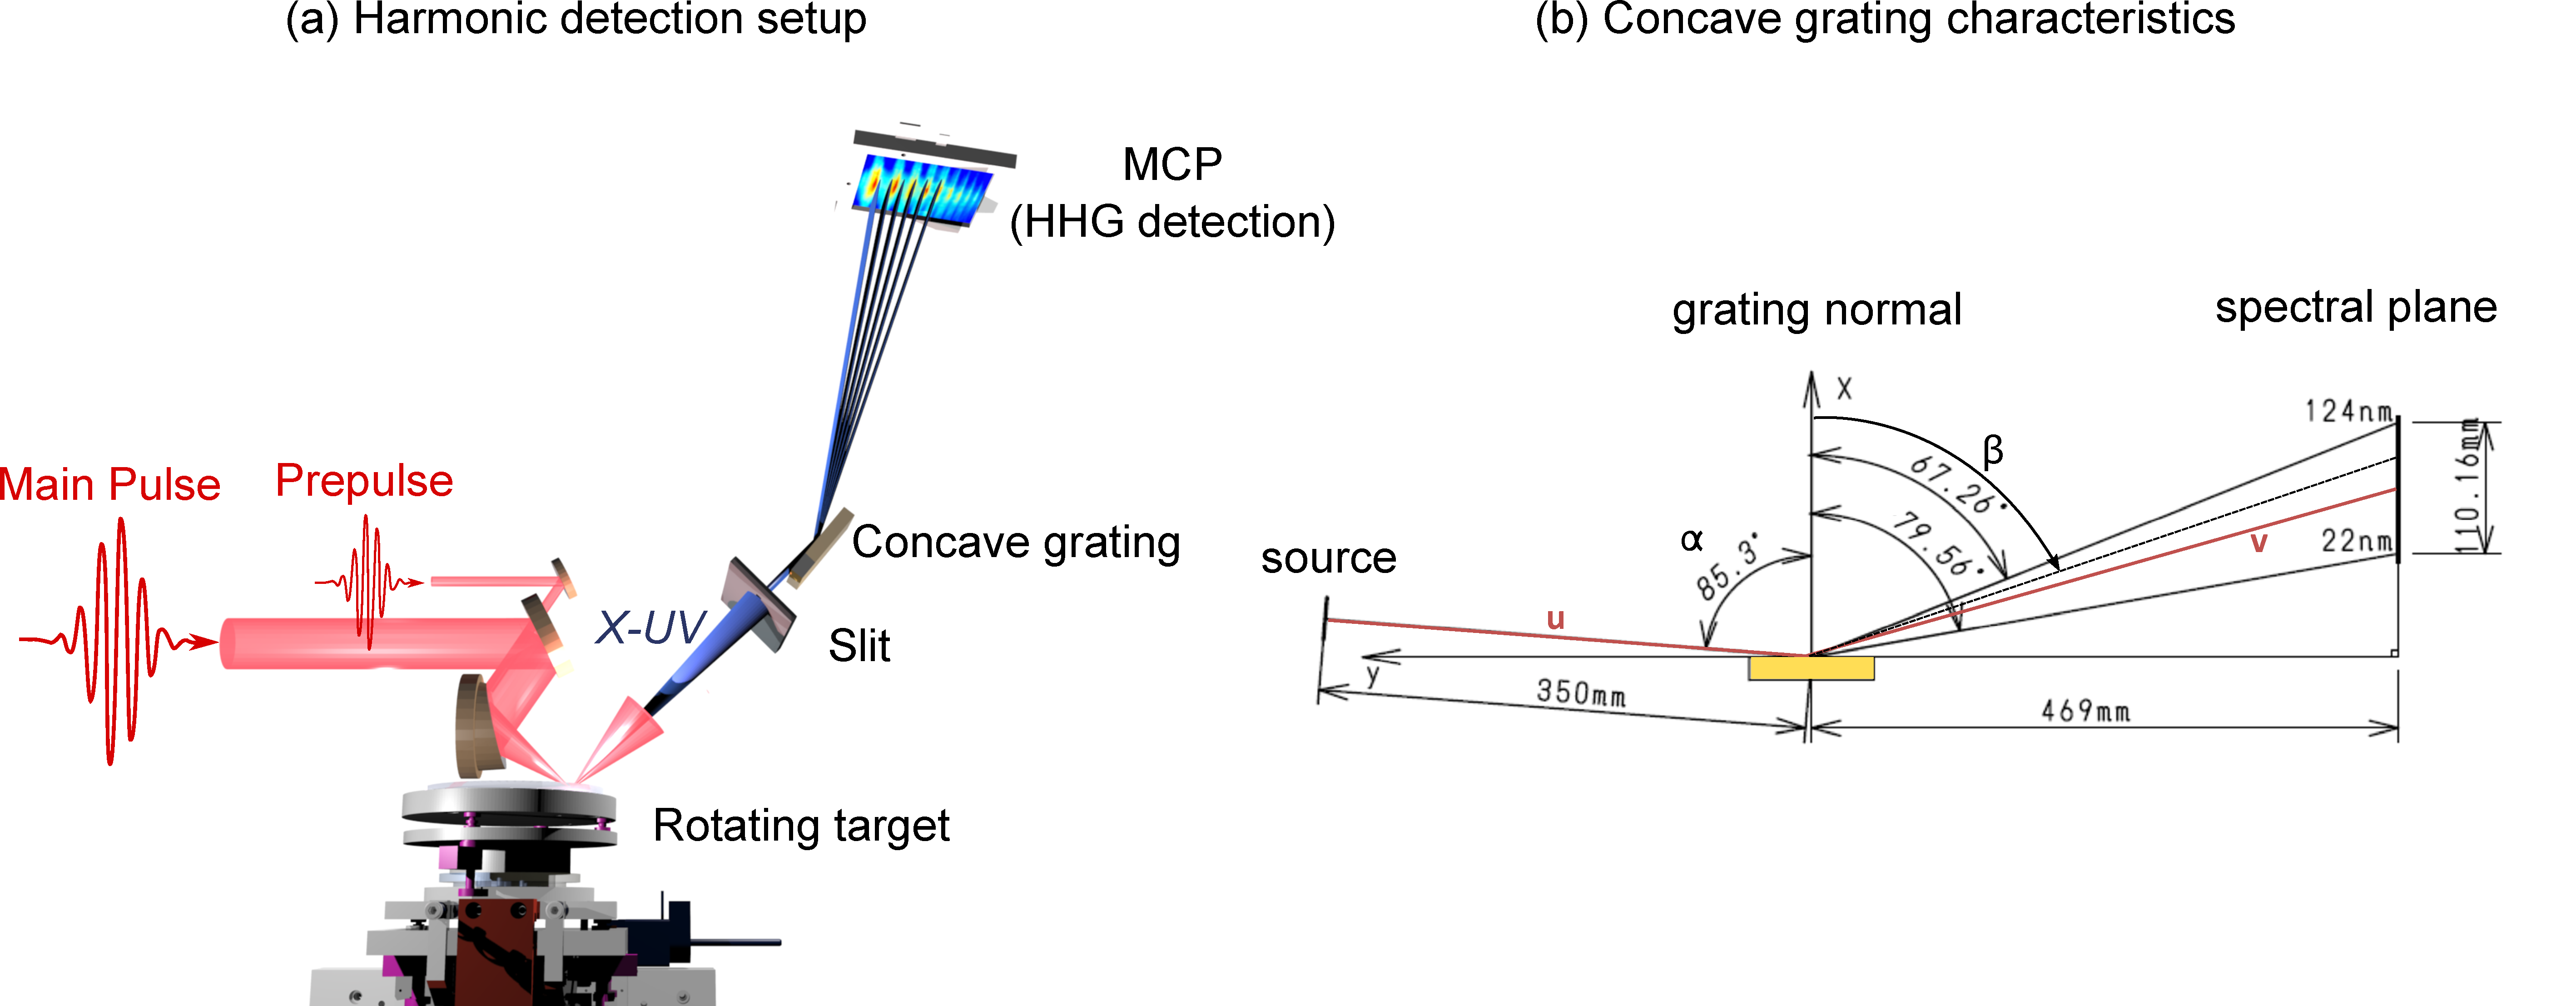
\includegraphics[width =1.1\textwidth]{../chapitre6/images/SETUP_hhg.pdf}}
\caption{\label{SETUP_hhg}(a) Experimental setup for HHG detection (b) spherical grating (\textit{Hitachi} 001-0639) for home-made spectrometer. The MCP is placed in the spectral plane and imaged using a triggered CCD.}
\end{figure}

\noindent The spherical grating was installed with respect to the focal spot in the configuration represented in Fig~\ref{SETUP_hhg}(b), that is to say $469$mm from the focal spot in the specular direction. In the direction orthogonal to propagation, the beam is diverging. The resulting X-UV spectrograph is recorded using a single-stack MCP\footnote{Micro-channel Plate: high-voltage photomultiplier micro-array for the detection of single photons with a wavelength below 120nm}(\textit{Photonis}) continuously biased at 1kV (amplification gain of $\sim 10^5$). The MCP has an effective detection area of H$\times$W = $75\times 93$mm. A P46 phosphor screen also biased at 1kV is stacked to the MCP. Its decay time is on the order of $100\,\mathrm{ns}$, which enables recording the MCP signal at 1kHz refresh rate.\\

\noindent We define $x$ and $y$ as the local spatial coordinates respectively in the horizontal and vertical MCP image plane. After the optical imaging system has been properly calibrated, we transform $y$ from mm to rad dividing its value by the quantity $u +v$ [mm] corresponding to the averaged propagation distance of the beam from the source to the detection plane. In doing this, we assume that $v$ is independent of $\lambda$, which yields a calibration error of 2\%. To transform $x$ from mm to wavelength, we used the diffraction relation:
$$
\sin \alpha + \sin \beta = \lambda \sigma_0
$$

\noindent where $\alpha =85.3^{\circ}$, $67.3^{\circ} \le \beta \le 80^{\circ}$ are defined in Fig~\ref{SETUP_hhg}(b), $\lambda$ is the wavelength and $\sigma_0 = 1/600\,\mathrm{mm}$ the  groove density.\\

\noindent Also represented in Fig~\ref{SETUP_hhg}(a), is the possibility of adding  a prepulse, aligned collinear to the main pulse through a holed mirror, in order to generate a controlled preplasma with intensity $\sim 10^{14}\,\mathrm{W/cm^2}$. Full details on the experimental chamber and 
beam characteristics have already been discussed in Chapter~\ref{chapter:Overall presentation of the laser system}.


\subsection{From harmonic emission time to CWE basic properties}\label{subsection:CWE emission time}

The 1D  Brunel model used to calculate the electron trajectories at the surface of the plasma is described in details in Section~\ref{section:Brunel absorption mechanism}. Here, we use this model to highlight some basic properties of CWE.
A more detailed description of this model can also be found in~\cite{TheseArnaud,TheseCedric}. We recall the equation of motion for an electron $i$ starting its motion at $t >t_i$:

\begin{equation}
\frac{d(\gamma_e v_e)}{dt} = -a_0[\bar{E}(t)-\bar{E}(t_i)]
\label{electron_i_equation}
\end{equation}

\noindent where $\gamma_e$ is the relativistic gamma factor of the electron, $v_e$ its velocity, and $a_0$ the normalized electric field amplitude. We solve this equation for every laser cycle, and every electron returning to the plasma bulk is considered ballistic past the critical density. The electron crossing trajectories overall describe a caustic in time, which for a given optical cycle, is defined by the relation:

\begin{equation}
x_c(t) = \min_{i} [v_i(t_{ri})(t-t_{ri})]
\end{equation}

\noindent where $t_{ri}$ defines the time at which the i$^{th}$ electron crosses the critical density, and $v_{ri}$ its corresponding velocity. 

\begin{figure}[H]
\makebox[0.95\textwidth][c]{
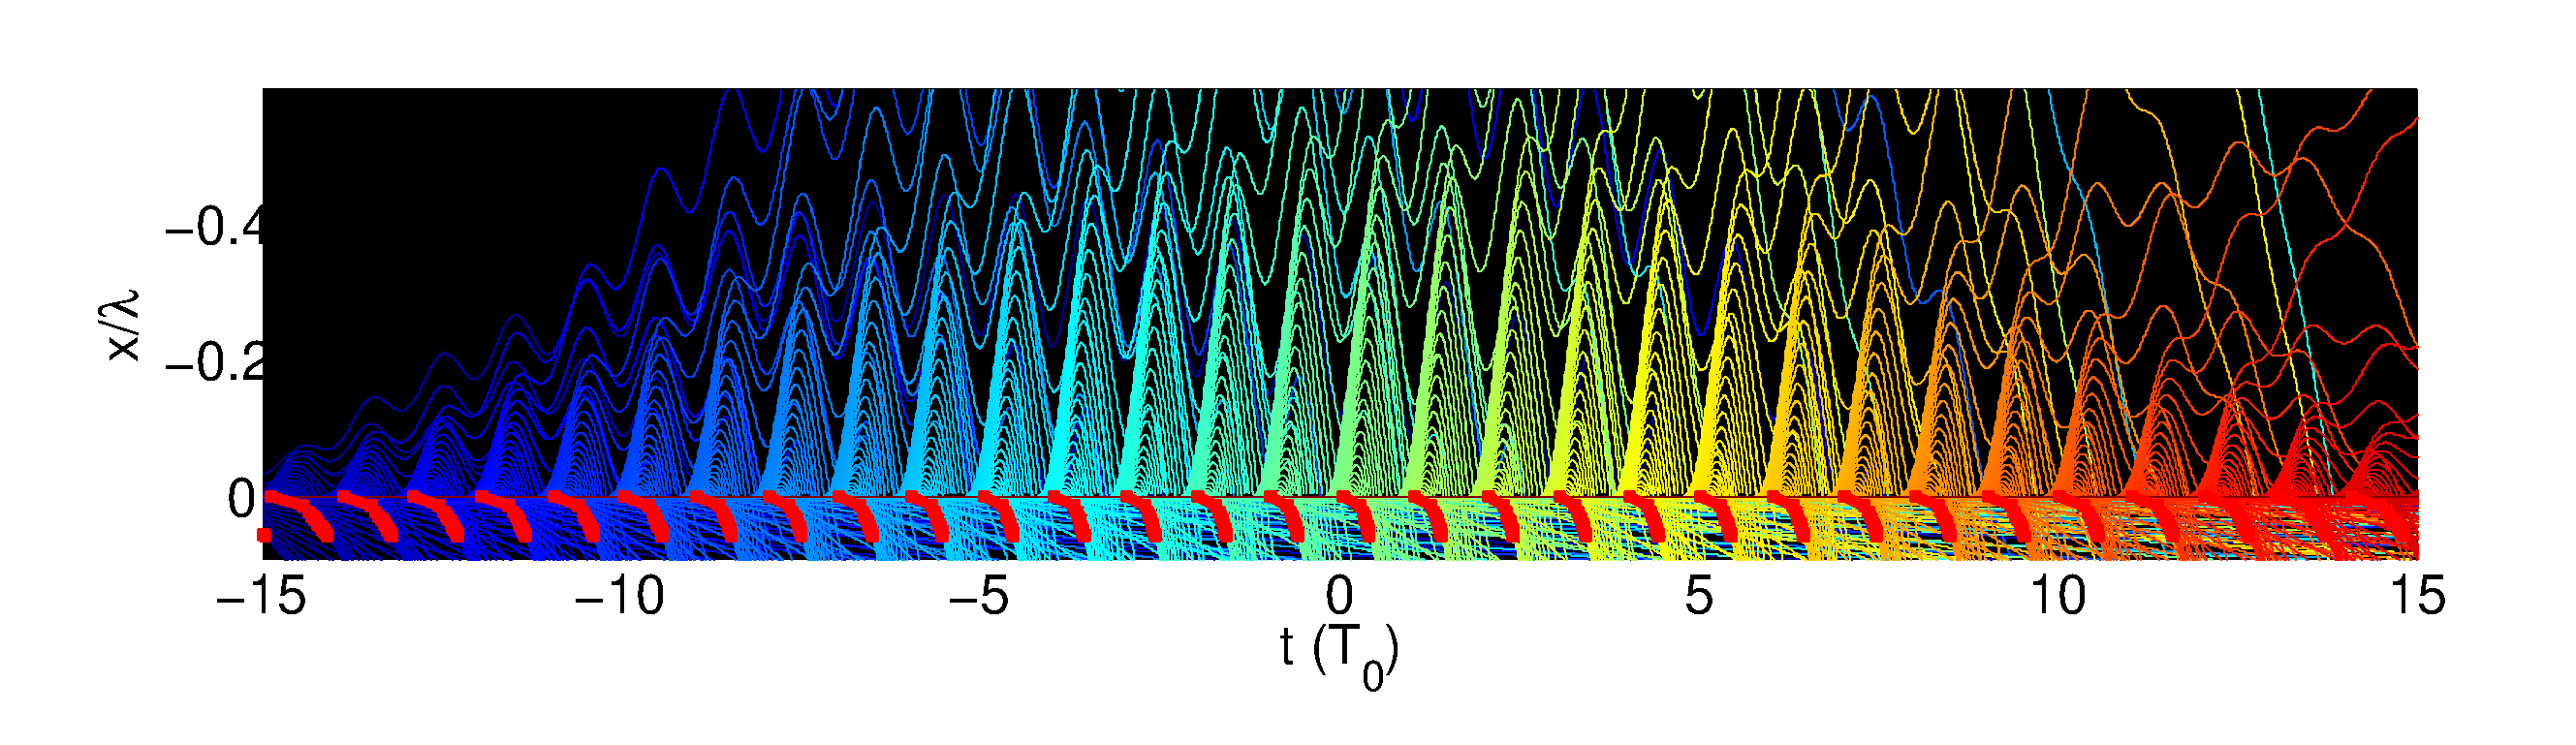
\includegraphics[width =1.1\textwidth]{../chapitre6/images/excursionsAndemissionCaustics.pdf}}
\caption{\label{excursionsAndemissionCaustics} Trajectories of Brunel electrons in vacuum for a $30\,\mathrm{fs}$ Gaussian pulse, $a_0 = 1$ and a gradient length $L = \lambda/100$. Each laser period, electrons are pulled out of and back into the plasma where trajectories cross. The "crossing" time is represented by the red caustics in the $x<0$ region ($x=0$ defines the critical surface).}
\end{figure}

\noindent This is well described in~\cite{thaury2010high} where it is shown that $x_c(t)$ can be approximated by a quadratic function of time.
The retrieved $x_c$ values in the case $a_0 = 1$ are plotted in red in Fig~\ref{excursionsAndemissionCaustics} as an illustration. 
Once $x_c$ is retrieved, we can calculate the so-called emission times of the harmonics. In other words, this is equivalent to provide information on the spectral phase of each emitted frequency. Indeed, we saw in section~\ref{section:Brunel absorption mechanism} how an overdense plasma submitted to an electronic perturbation emits coherent light at a frequency $\omega_p(x) = \sqrt{e^2 n_e(x)/(m_e \epsilon_0)}$, where $x$ is the position where the plasma density equals $n_e(x)$. Therefore, the emission time $t_e$ of the n$^{th}$ harmonic, for a given optical cycle, is defined by the relation:
$$
\omega_p[x_c(t_e)] = n \omega_0
$$

\noindent In Fig~\ref{fig:EmissionTimeComparison} we calculate the emission times for a laser intensity of respectively $a_0 = 0.2$ and $a_0 = 1$. One can clearly see that the relative emission delay from one optical cycle to the next decreases with increasing $a_0$. We can also show that this delay, also called \g{femtosecond chirp}, increases with the gradient scale length~\cite{TheseArnaud}.
This \g{femtosecond chirp} is a signature of CWE emission and will have a direct influence over the spectral width of the generated harmonics. This was very well described in previous  PhD work~\cite{TheseArnaud,theseAnto,malvache2013coherent,TheseCedric}.


\begin{figure}[H]
\centering
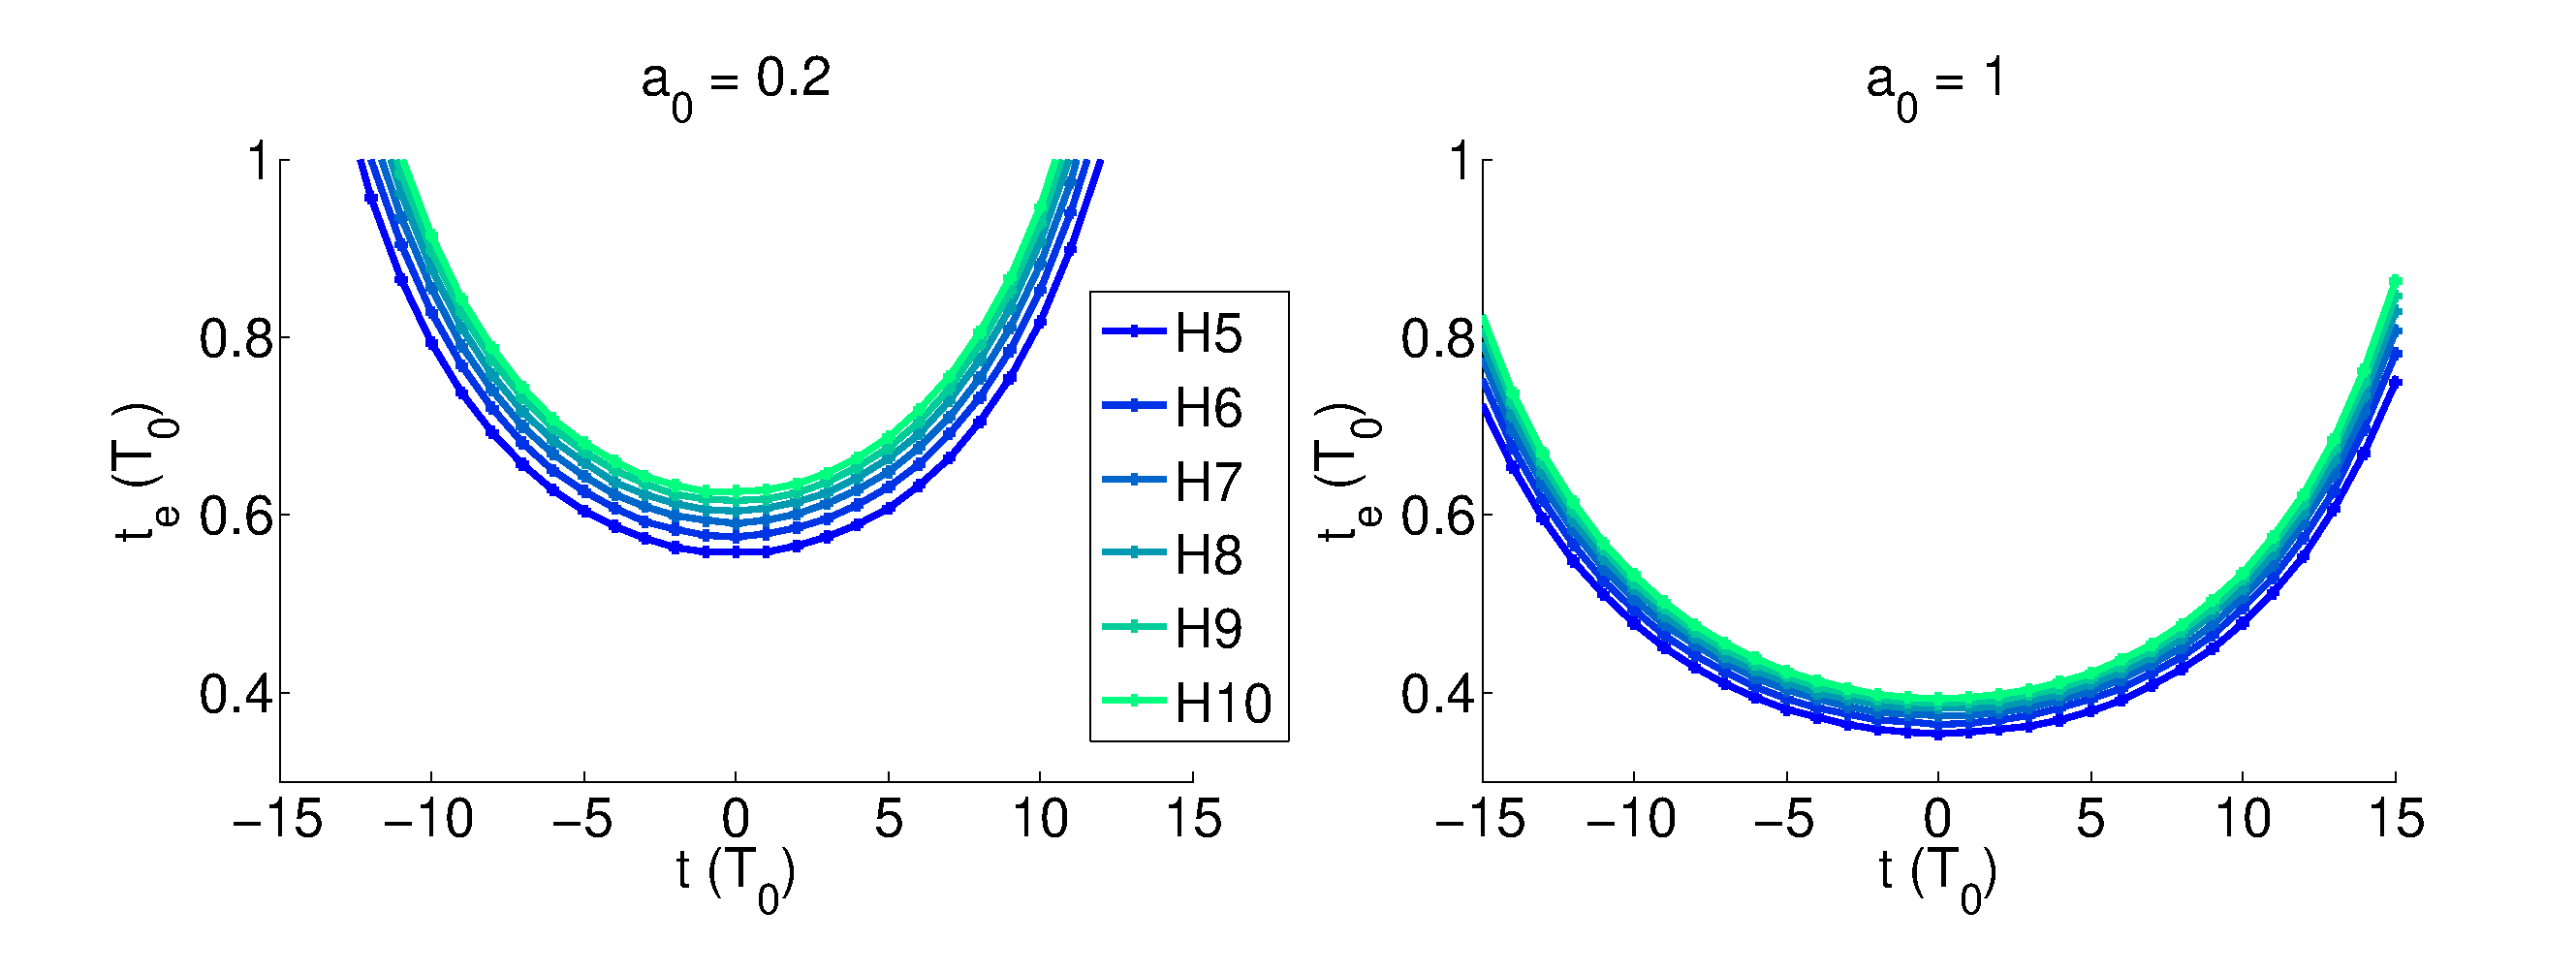
\includegraphics[width =\textwidth]{../chapitre6/images/EmissionTimeComparison.pdf}\\
\caption{\label{fig:EmissionTimeComparison} CWE emission time calculated using 1D Brunel model for harmonics 5 to 10, a Gaussian pulse of $30\,\mathrm{fs}$ duration, a gradient length $L= \lambda / 100$ and laser intensities of $a_0 = 0.2$ and $a_0 =1$ respectively.}
\end{figure}

\noindent Using the calculated emission times $t_e(n,.)$ for every optical cycle $n$ of the driving laser pulse, one can define the HHG spectrum as the coherent sum of each component $\omega \in [\omega(n_c)\ \ \omega(n_{max})]$ such that~\cite{TheseArnaud}:

\begin{equation}
E_{\text{HHG}}(\omega) = \sum_{n}A_n(\omega)\exp[i\omega(nT_0+t_e(n,\omega))]
\end{equation}

\noindent where $n$ denotes the optical cycle, $T_0$ the driving laser period and $A_n(\omega)$ the spectrum of the attosecond pulse generated during the $n^{th}$ optical cycle. This expression is quite explicit and it appears straightforward that in the ideal case where $t_e(.,\omega)$ would be independent of $n$ (i.e. perfect periodicity of the attosecond pulses emission), the corresponding spectral phase can be factorized in front of the sum and the harmonic spectra would be convolved by a purely Dirac comb. This corresponds to the minimum harmonic spectral width. 

\begin{figure}[H]
\centering
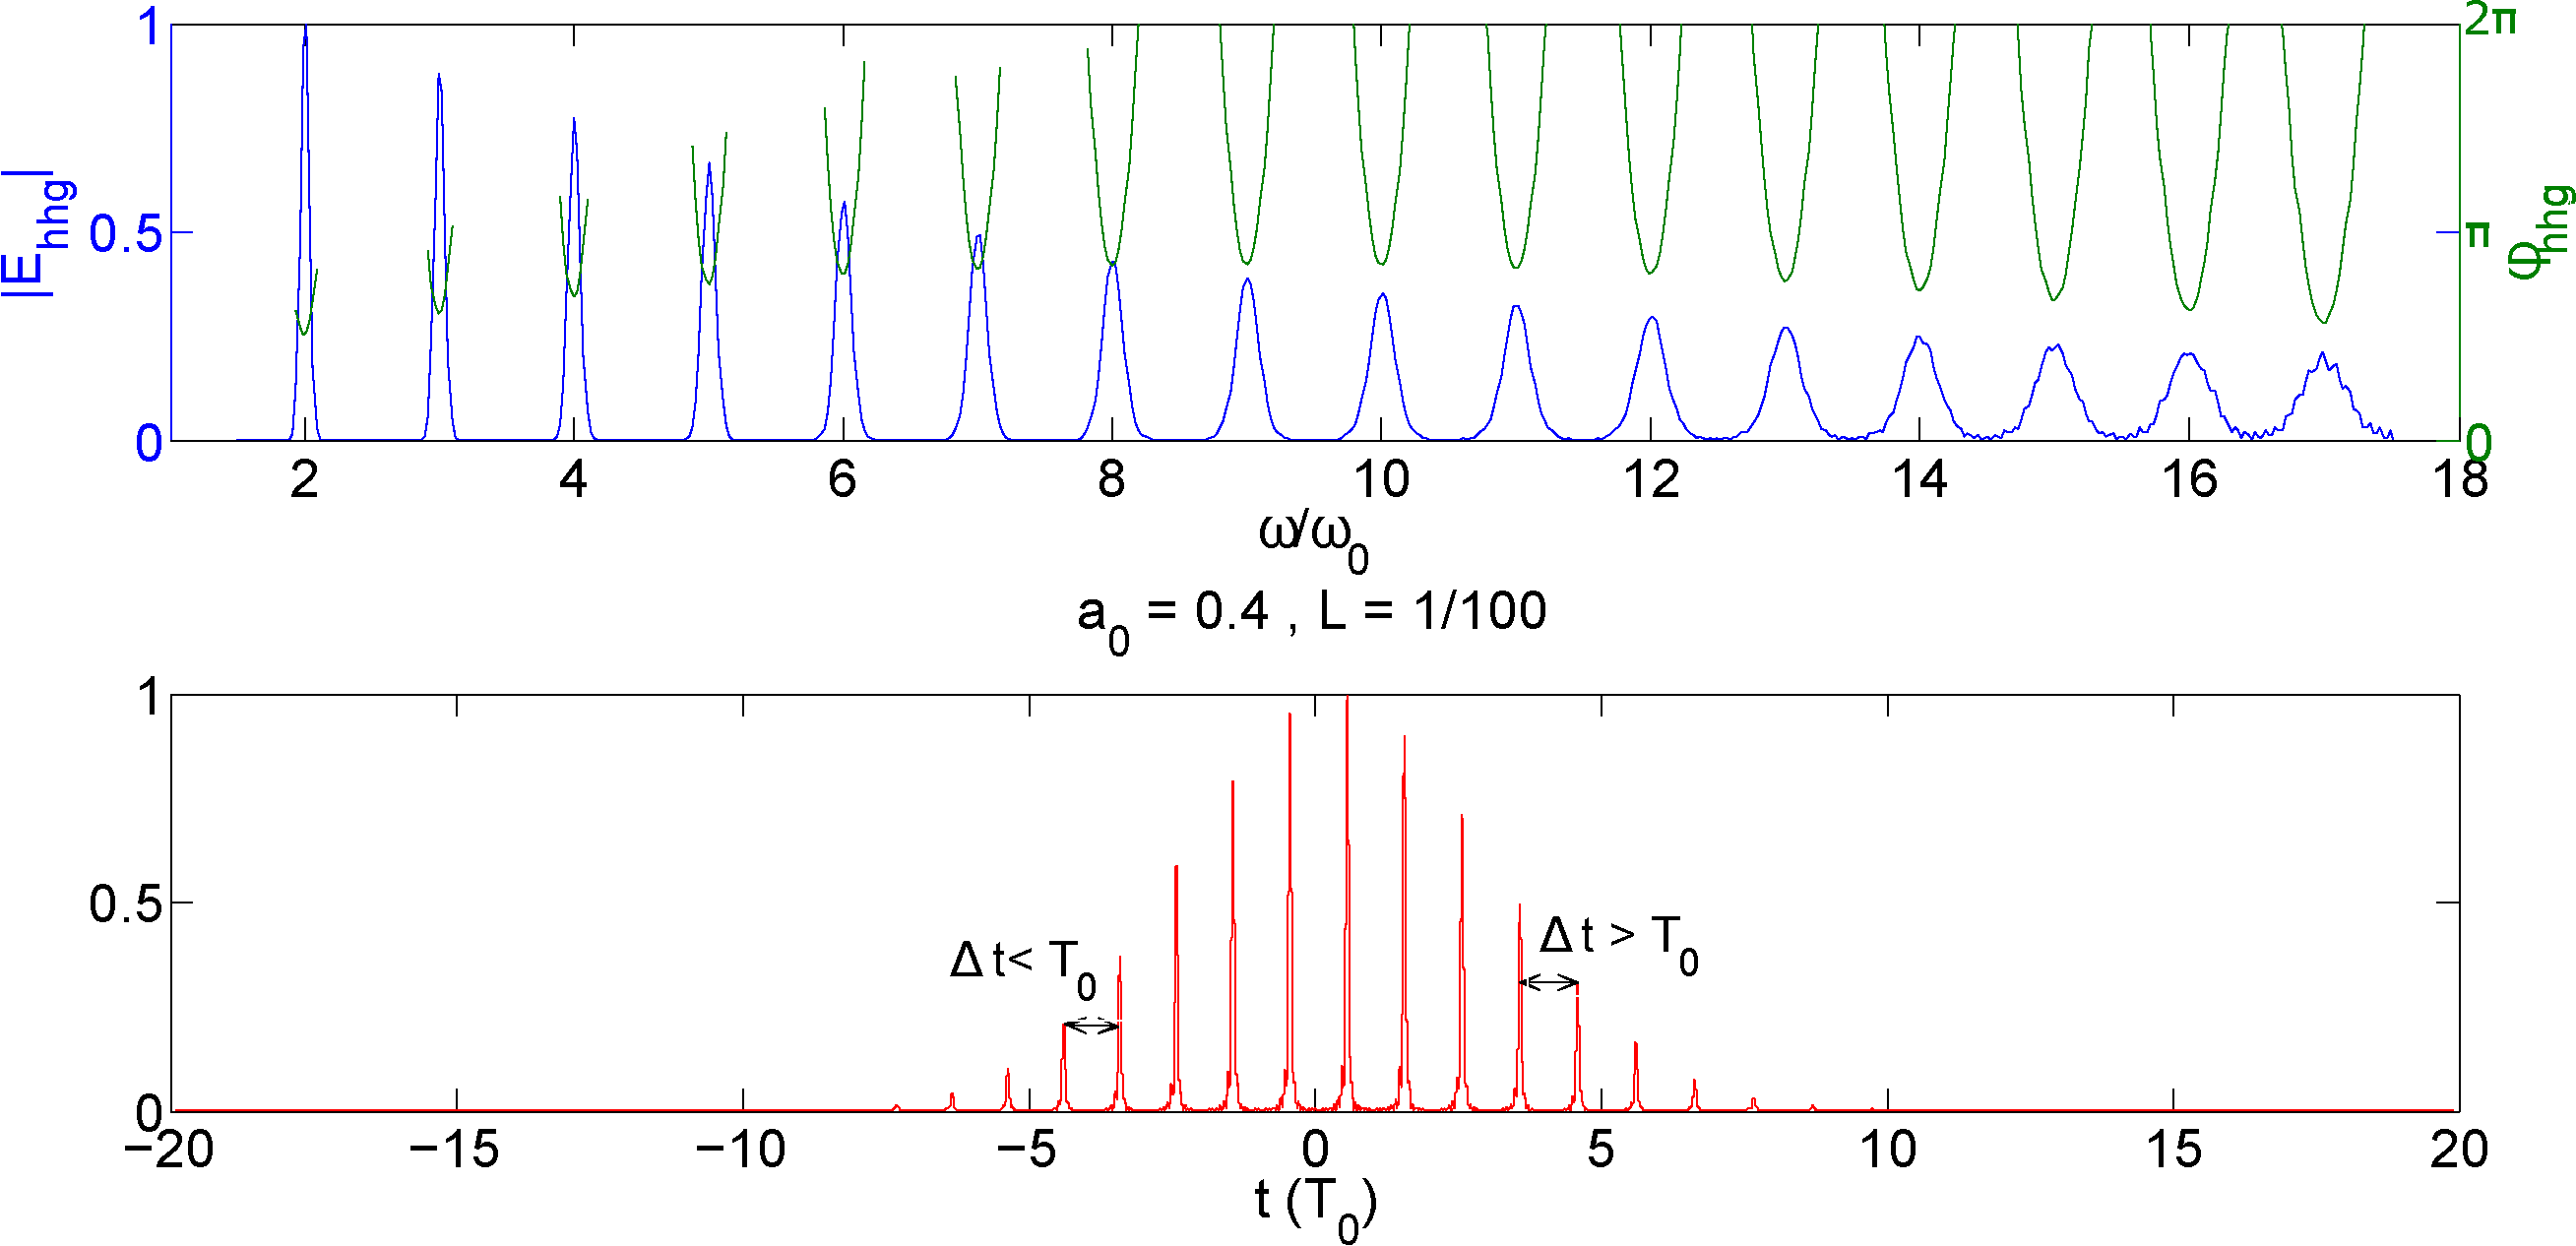
\includegraphics[width =\textwidth]{../chapitre6/images/hhg1DmodelExample.pdf}\\
\caption{\label{fig:hhg1DmodelExample} CWE emission spectral and temporal profile for a $30\,\mathrm{fs}$ Gaussian pulse, a gradient length $L= \lambda / 100$ and an intensity of $a_0 = 0.4$ }
\end{figure}

\noindent On the other hand, when $t_e(n,.)$ varies with $\omega$, each harmonic line broadens spectrally. When the driving laser pulse is compressed, the emission time varies from cycle to cycle, as represented in Fig~\ref{fig:hhg1DmodelExample} for $a_0 = 0.4$. We represent the intensity of the corresponding attosecond pulse train in the temporal domain, where we can see a variation in the train periodicity. This can be observed experimentally by chirping the driving laser pulse. Indeed, a positive chirp will shift the lower frequencies to the beginning of the pulse, and the higher frequencies to the end. As a consequence, the change of instantaneous period as the pulse generates harmonics can compensate the intrinsic femtosecond chirp. This will lead to spectrally narrow harmonics, as clearly demonstrated in Fig~\ref{fig:ChitpInfluence} where we used the Dazzler to introduce a second order chirp of $\phi^{(2)} = 400\,\mathrm{fs^2}$ ($\xi = 0.6$)\footnote{The normalized chirp is define by $\xi = \phi^{(2)}/\sigma^2$, defined for a Gaussian pulse of intensity $\propto e^{-t^2/(2\sigma^2)}$} in the driving laser.

\begin{figure}[H]
\centering
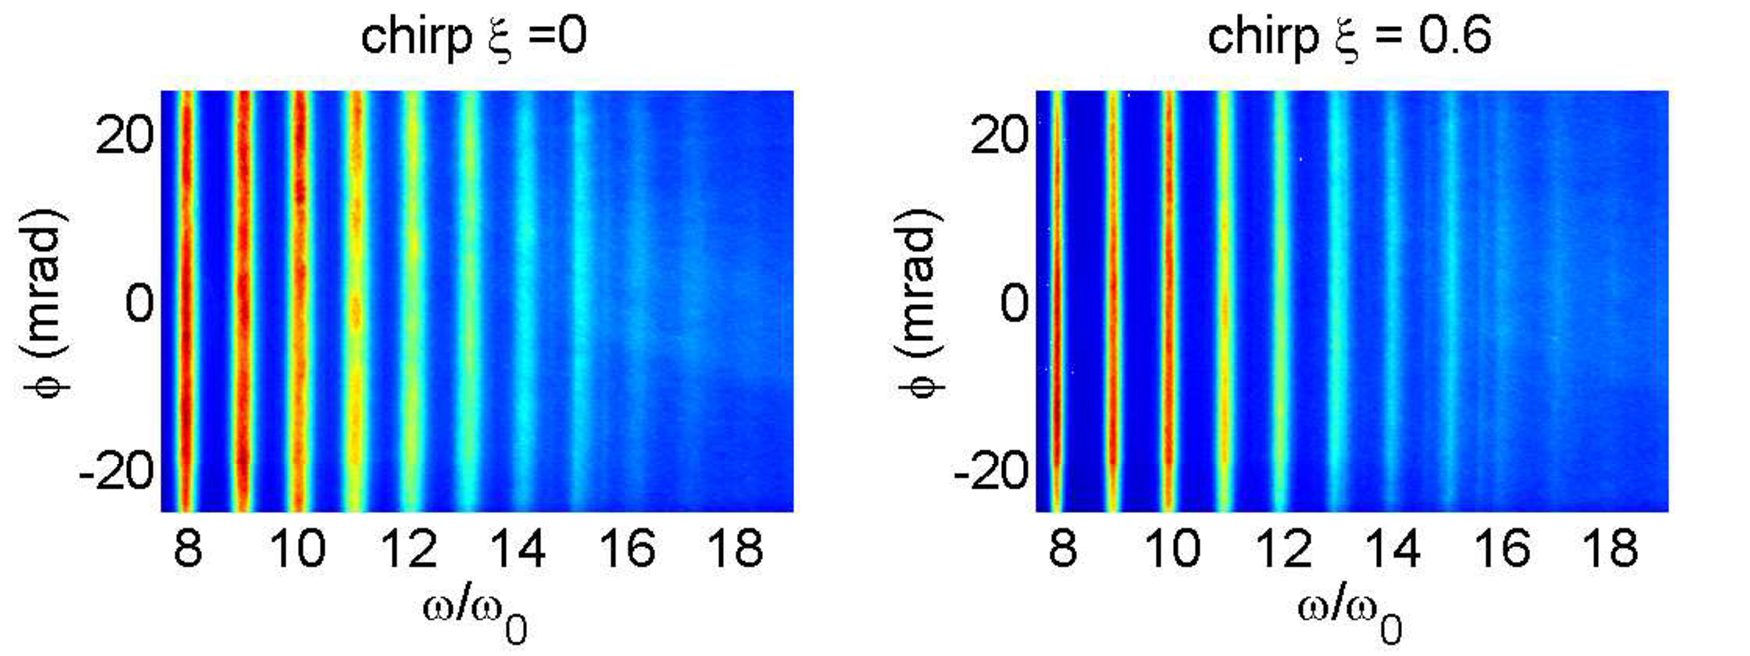
\includegraphics[width =\textwidth]{../chapitre6/images/ChitpInfluence.pdf}\\
\caption{\label{fig:ChitpInfluence} CWE experimental  spectra for a compressed $26\,\mathrm{fs}$ pulse with $a_0 = 0.4$(left caption) and with a normalized order chirp of $\xi = 0.6$ (right panel)}
\end{figure}

\subsection{Harmonic coherence properties}\label{subsection:Harmonic spatial properties}

The generated X-UV source conserves the coherence properties of the initial laser pulse. In other words, the X-UV generation plane defined by the target surface can be pictured as the coherent superposition of infinitesimal sources with a well-defined phase relation between them. The wavefront is convex with respect to the direction of propagation, which is to be expected: considering that the intensity at the center of the driving laser is higher than on the edges, the emission therefore occurs ``sooner'. This spatially dependent delay of harmonic emission corresponds to a CWE wavefront curvature~\cite{TheseArnaud}. In other words, if the harmonic beam were to be approximated by a Gaussian beam as represented on Fig~\ref{fig:GaussianBeamDef0}, its waist (position where the spatial phase is flat) would be located before the focusing plane of the driving IR laser. Any modification of the emission time at focus (linked to a change of gradient length, compression, laser intensity) therefore translates into variations of the beam divergence and can be compensated by adjusting the driving laser defocus~\cite{TheseArnaud,TheseCedric}.


\begin{figure}[H]
\centering
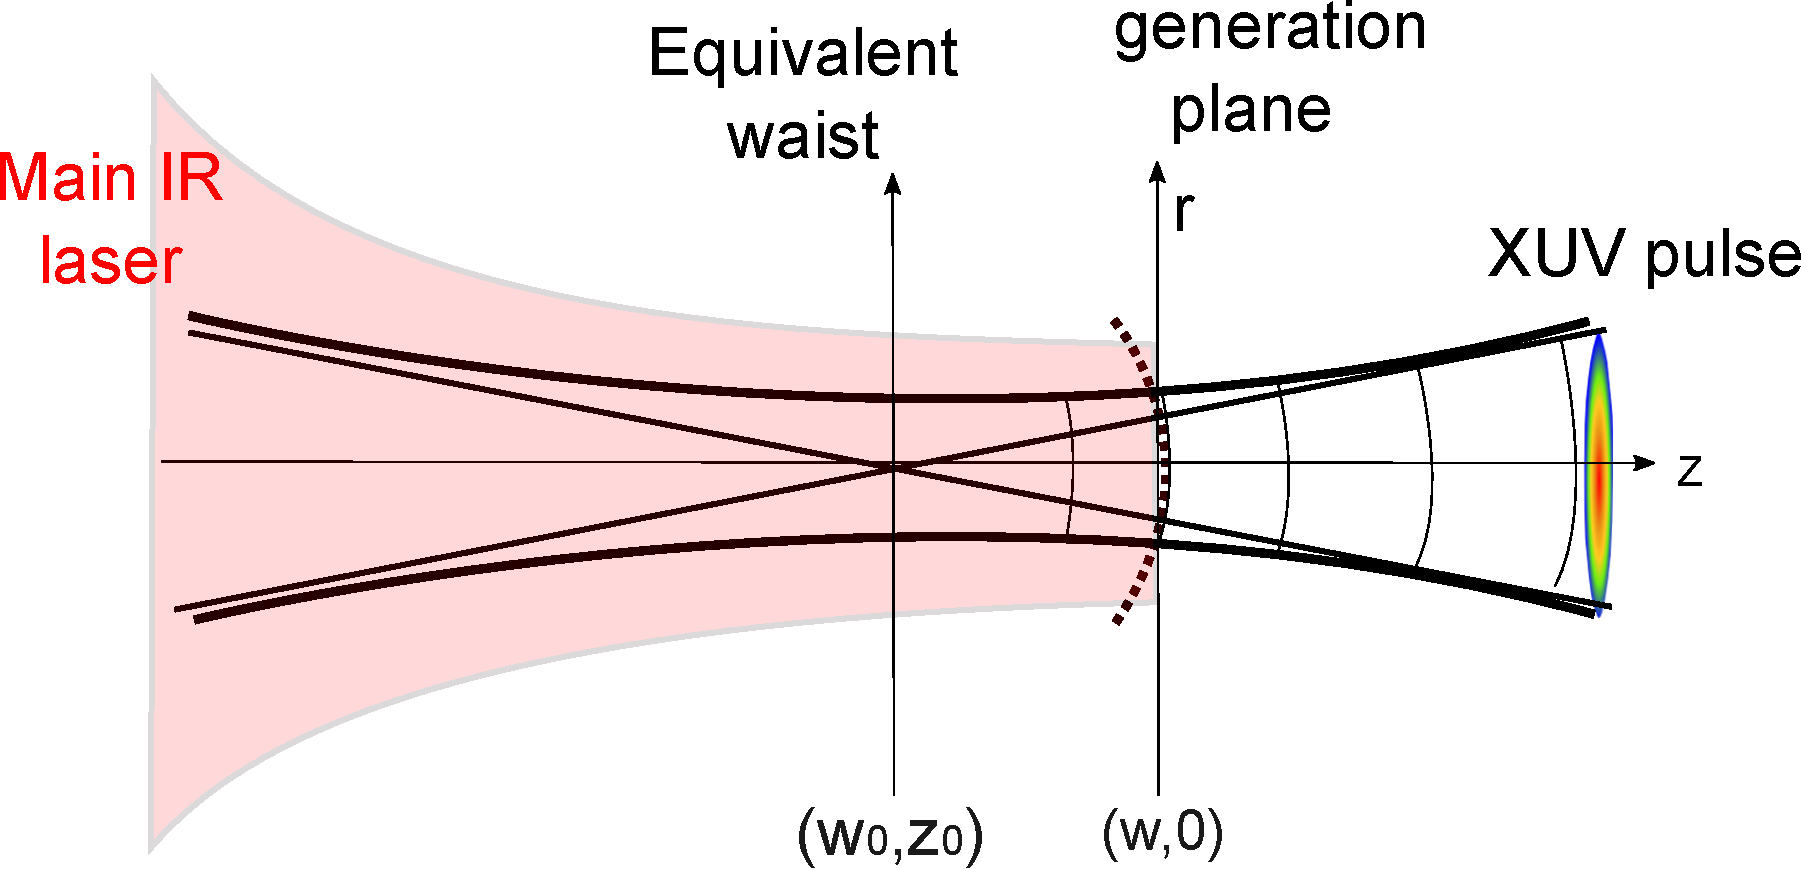
\includegraphics[width =10cm]{../chapitre6/images/GaussianBeamDef.pdf}\\
\caption{\label{fig:GaussianBeamDef0} Gaussian beam representation for X-UV pulse generated at the focus of a driving IR femtosecond pulse. The "generation plane" refers to the solid-target surface.}
\end{figure} 

\noindent The divergence for harmonic $n$, of frequency $\lambda_0/n$ and waist $w_{0,n}$ is therefore:
\begin{equation}
\label{eq:HHGdivDef}
\Delta_{n} = \frac{\lambda_0}{n\pi w_{0,n}} = \frac{\lambda_0}{n\pi w_{n}}\sqrt{1+\frac{z_{0,n}^2}{Z_{R,n}^2}} 
\end{equation}

\noindent where $w_n$ is the waist in the plane of generation, $z_{0,n}$ the distance from the waist position as represented in Fig~\ref{fig:GaussianBeamDef0} and $Z_{R,n}$ the Rayleigh length. \\

%\subsection{Harmonic coherence properties}\label{subsub:Harmonic influence coherent properties}

\noindent We reproduce a simple original experiment which was the first to highlight the coherence properties of the X-UV emission~\cite{thaury2008coherent}. It consists in adding a transmission mask in the form of a comb, as drawn in Fig~\ref{fig:GratingExperiment}(a) in the collimated incident laser beam. As a result of diffraction, the beam splits into several sources separated by $4\,\mathrm{\mu m}$ as determined by the image of the focus shown on Fig~\ref{fig:GratingExperiment}(b-c), where only the 3 central diffraction orders intense enough to be detected on the camera are represented.
\begin{figure}[H]
\centering
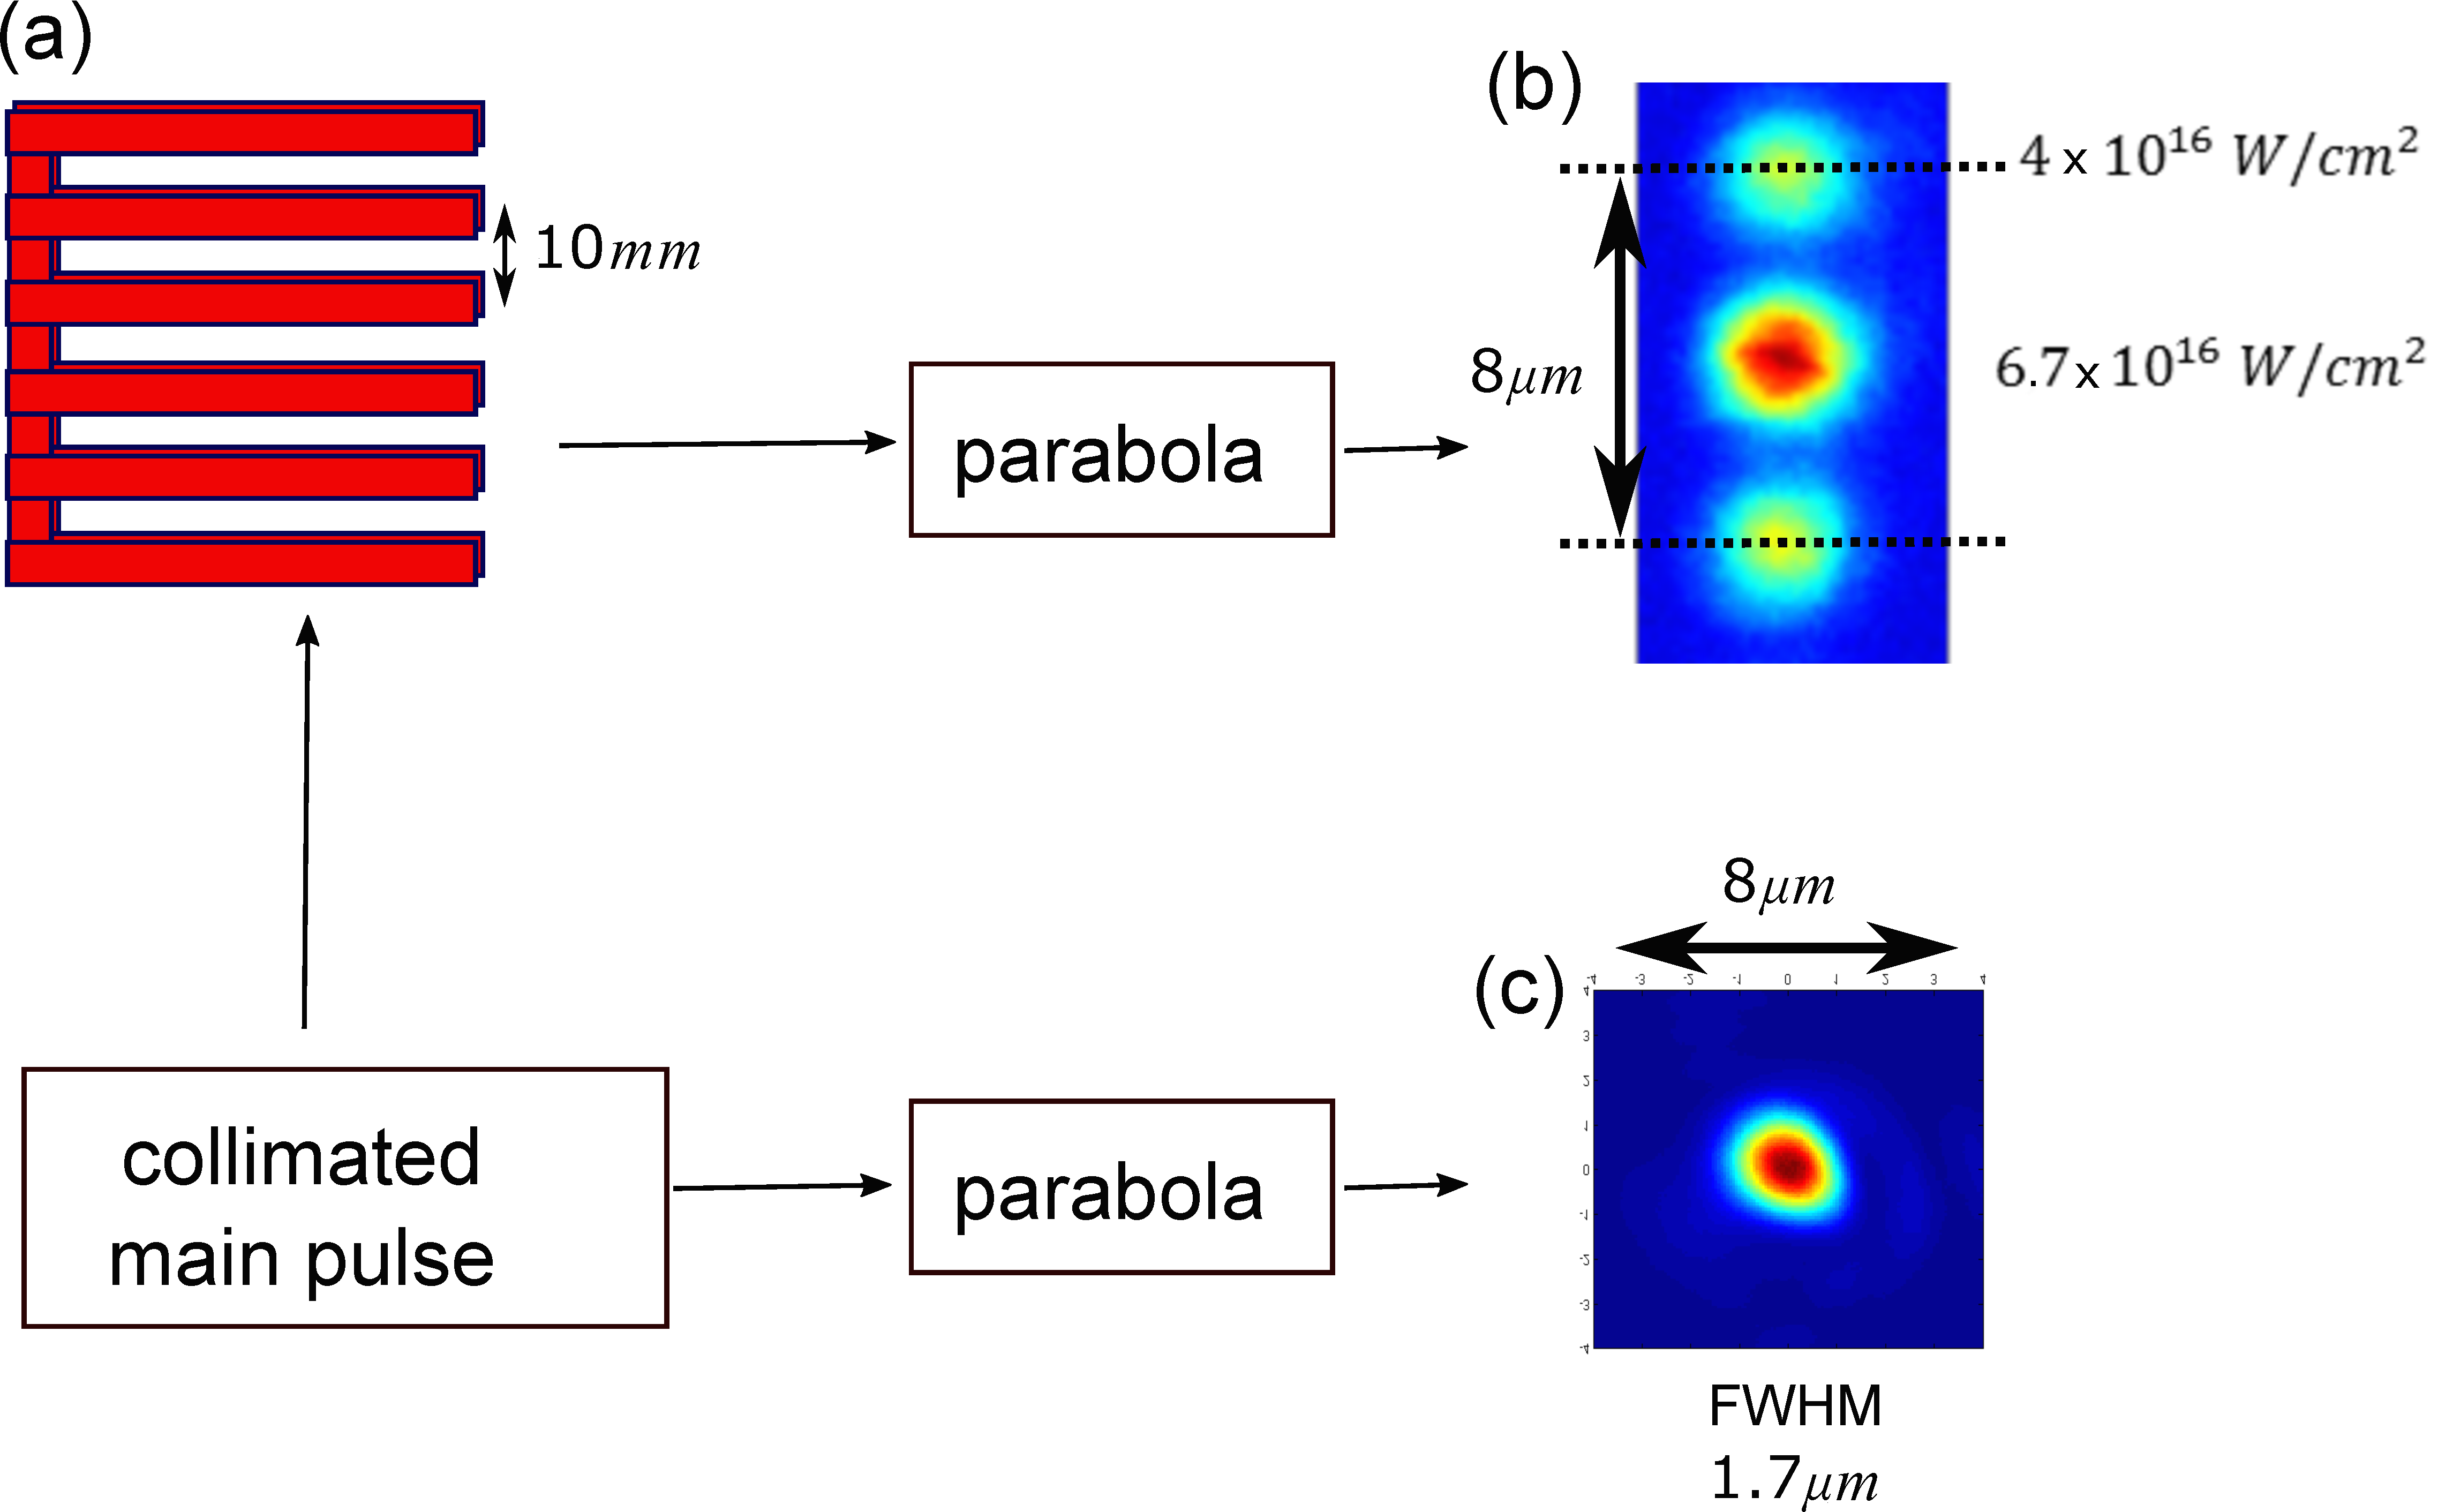
\includegraphics[width  =\textwidth]{../chapitre6/images/GratingExperiment.pdf}\\
\caption{\label{fig:GratingExperiment} A transmission mask~(a) is inserted into the collimated IR driving laser prior to the parabola. At focus, the main focal spot~(c) splits into 3 replicas~(b) relatively seperated out by $4\,\mathrm{\mu m}$ as a result of diffraction.}
\end{figure}

\noindent The central spot intensity is evaluated to be $\sim 6.7\times 10^{16}\,\mathrm{W/cm^2}$, and a little over half for the satellites. This will lead the harmonics to interfere constructively in the far field. In the result presesented in Fig~\ref{fig:GratingExperiment-2}, we performed a vertical Fourier transform of the HHG image detected on the MCP, and defined the vertical axis by $r_1= \lambda f_{\theta}$. This way, the vertical axis is homogeneous to a distance and the first-order diffraction should be located at $r_1 =4\,\mathrm{\mu m}$ which corresponds to the focal spot spacing measured in Fig~\ref{fig:GratingExperiment}(b) (cf Appendix~\ref{ch:Investigation of a coherent source}).
The result of this operation is represented in Fig~\ref{fig:GratingExperiment-2} for harmonics 10 to 12. The side band located at $4\mathrm{\mu m}$ is a clear indication the three sources are individually generating X-UV radiation even when the laser is out of focus.
\noindent The lines are slightly larger for H10 then they are for H12. This is to be expected and corresponds to a waist $w_n$ (using the same notation as in Eq~\ref{eq:HHGdivDef}) that decreases with the emission wavelength. The frequencies are more effectively generated in the zone of higher intensity as described in Appendix~\ref{ch:Investigation of a coherent source}.


\begin{figure}[H]
\centering
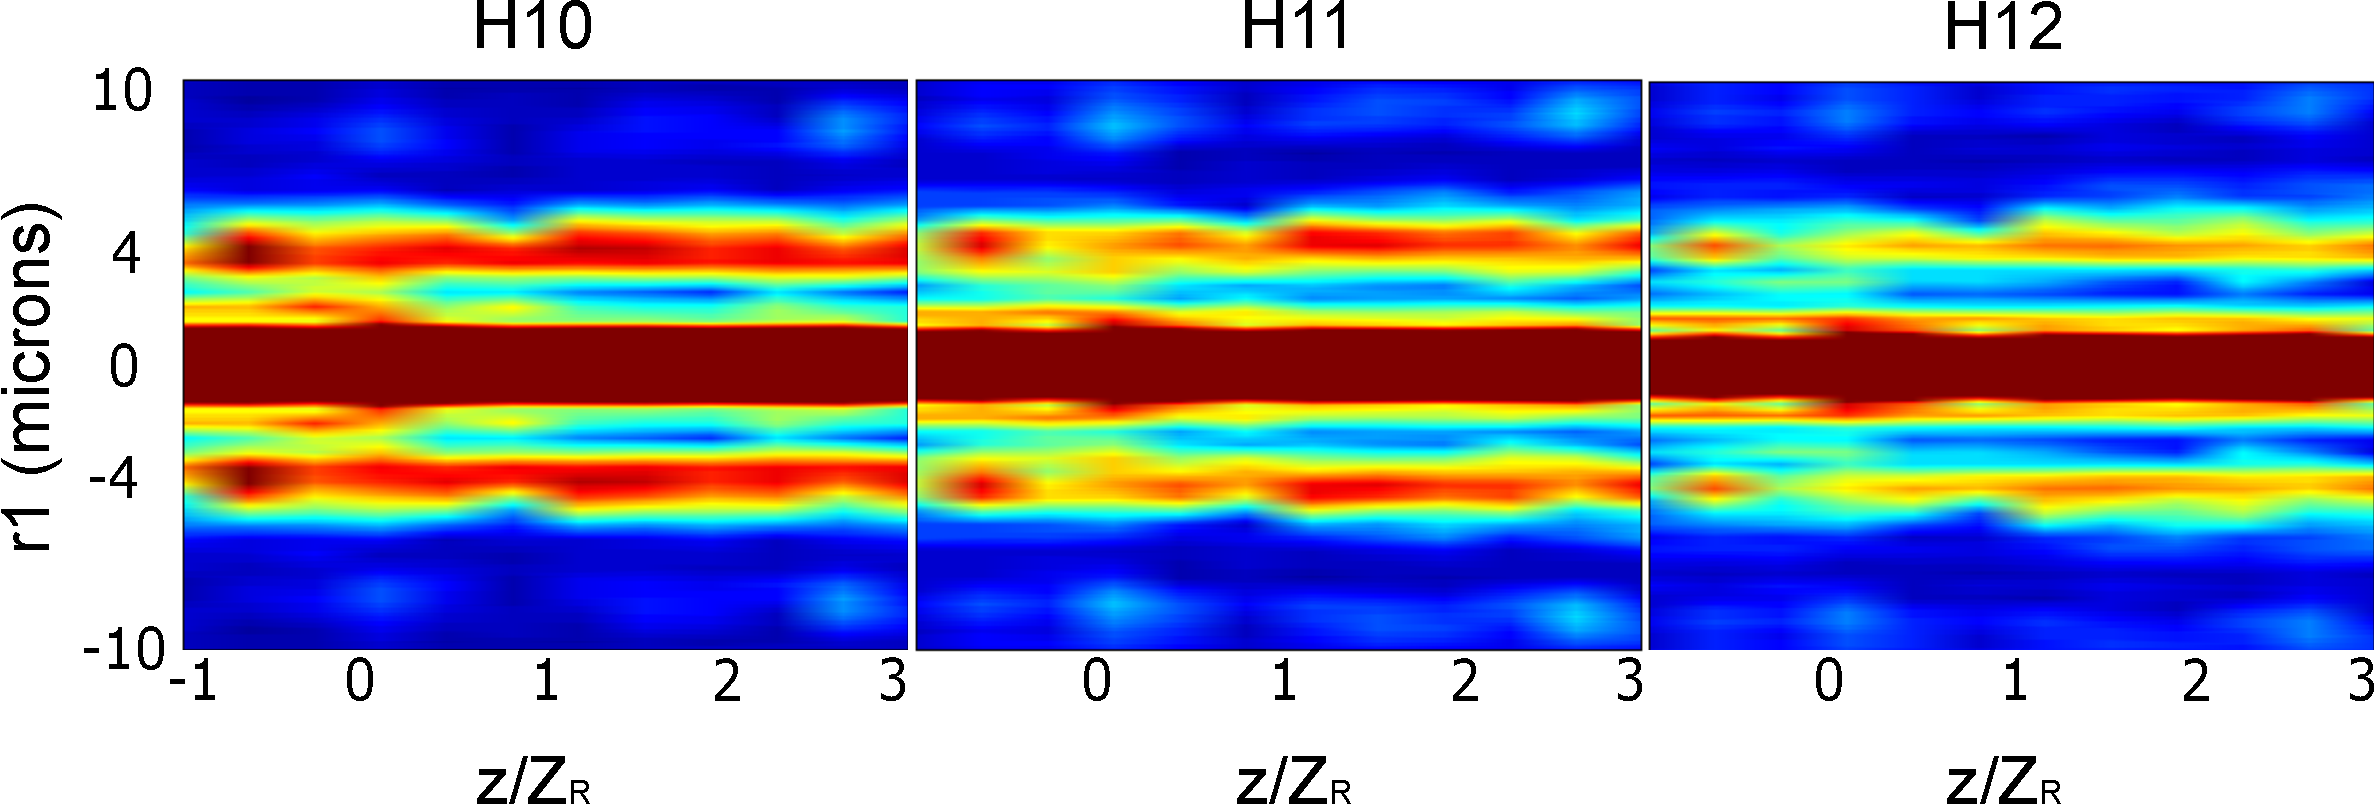
\includegraphics[width =\textwidth]{../chapitre6/images/GratingExperiment-2.pdf}\\
\caption{\label{fig:GratingExperiment-2} Retrieved spatial separation $r_1$ between individual HHG sources generated on target as a function of laser defocusing. The result is given for three different harmonic orders (H10, H11 and H12). The $0^{th}$ order was intentionally saturated to highlight the side bands.}
\end{figure}

\subsection{Influence of gradient scale length on HHG} \label{Influence of gradient scale length on harmonic generation}

As already explained in section~\ref{section:Harmonic plasma response to Brunel electrons}, the plasma scale length has a dramatic influence on the harmonic generation. In particular, the generation becomes inefficient for very long ($L >> \lambda/5$) or very short ($L<<\lambda/100$) plasma scale length. Observing the drop in harmonic generation efficiency with the gradient scale length is a rather simple experiment to conduct as it simply requires to degrade the laser contrast. On the other hand, observing the optimum in generation efficiency is rather challenging because it requires a very good control of the laser contrast. We saw in Section~\ref{chapter:Overall presentation of the laser system} how prepulses could very well emerge in a laser chain even in the presence of an XPW contrast filter because of non-linear effects. In Fig~\ref{fig:OptimumHHGgeneration}(a) we show how upgrading the laser chain contrast enabled us to observe an optimum CWE generation efficiency for $L/\lambda \sim 1/100$. 
Nevertheless, the laser intensity had to be kept at $a_0 \le 0.35$ for this optimum to be visible. Since we observed this optimum in PIC simulations for $a_0>0.35$, we conclude that unless the intensity of the main pulse is kept low, the target surface quality is sensitive to the coherent contrast of the laser.
In Fig~\ref{fig:OptimumHHGgeneration}(b), the gradient length in units of $\lambda$  was retrieved using SDI (described in section~\ref{ch:Measuring the gradient expansion}).
For the sake of comparison with what should be expected for the optimal gradient length, we performed a 2D PIC simulations using Epoch code~\cite{Arber:2015hc} with $a_0=0.4$ and Fig~\ref{fig:a0=0p4} shows the results of CWE efficiency for gradient scale lengths of respectively $L = \lambda/5, \lambda/10,\lambda/20,\lambda/40$ and $\lambda/80$.


\begin{figure}[H]
\centering
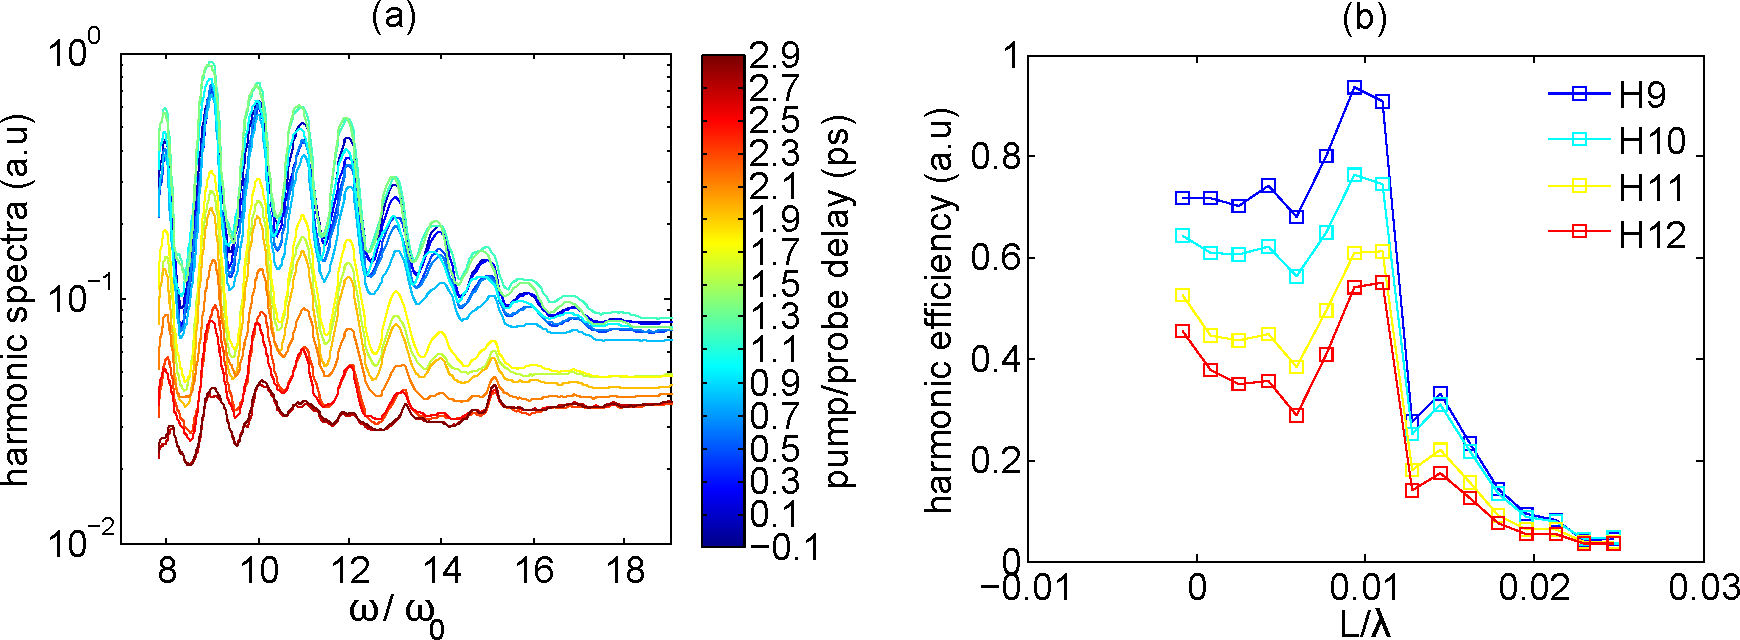
\includegraphics[width=\textwidth]{../chapitre6/images/OptimumHHGgeneration.pdf}\\
\caption{\label{fig:OptimumHHGgeneration}(a) Experimental  harmonic spectra integrated along the vertical direction at different prepulse delays indicated in the colorscale. (b) Corresponding relative intensity of harmonics 9 to 12.  Experimental conditions: $30\,\mathrm{fs}$ laser pulse with $a_0=0.35$. The prepulse intensity is $1.3 \times 10^{14}\,\mathrm{W/cm^2}$.}
\end{figure}


\begin{figure}[H]
\centering
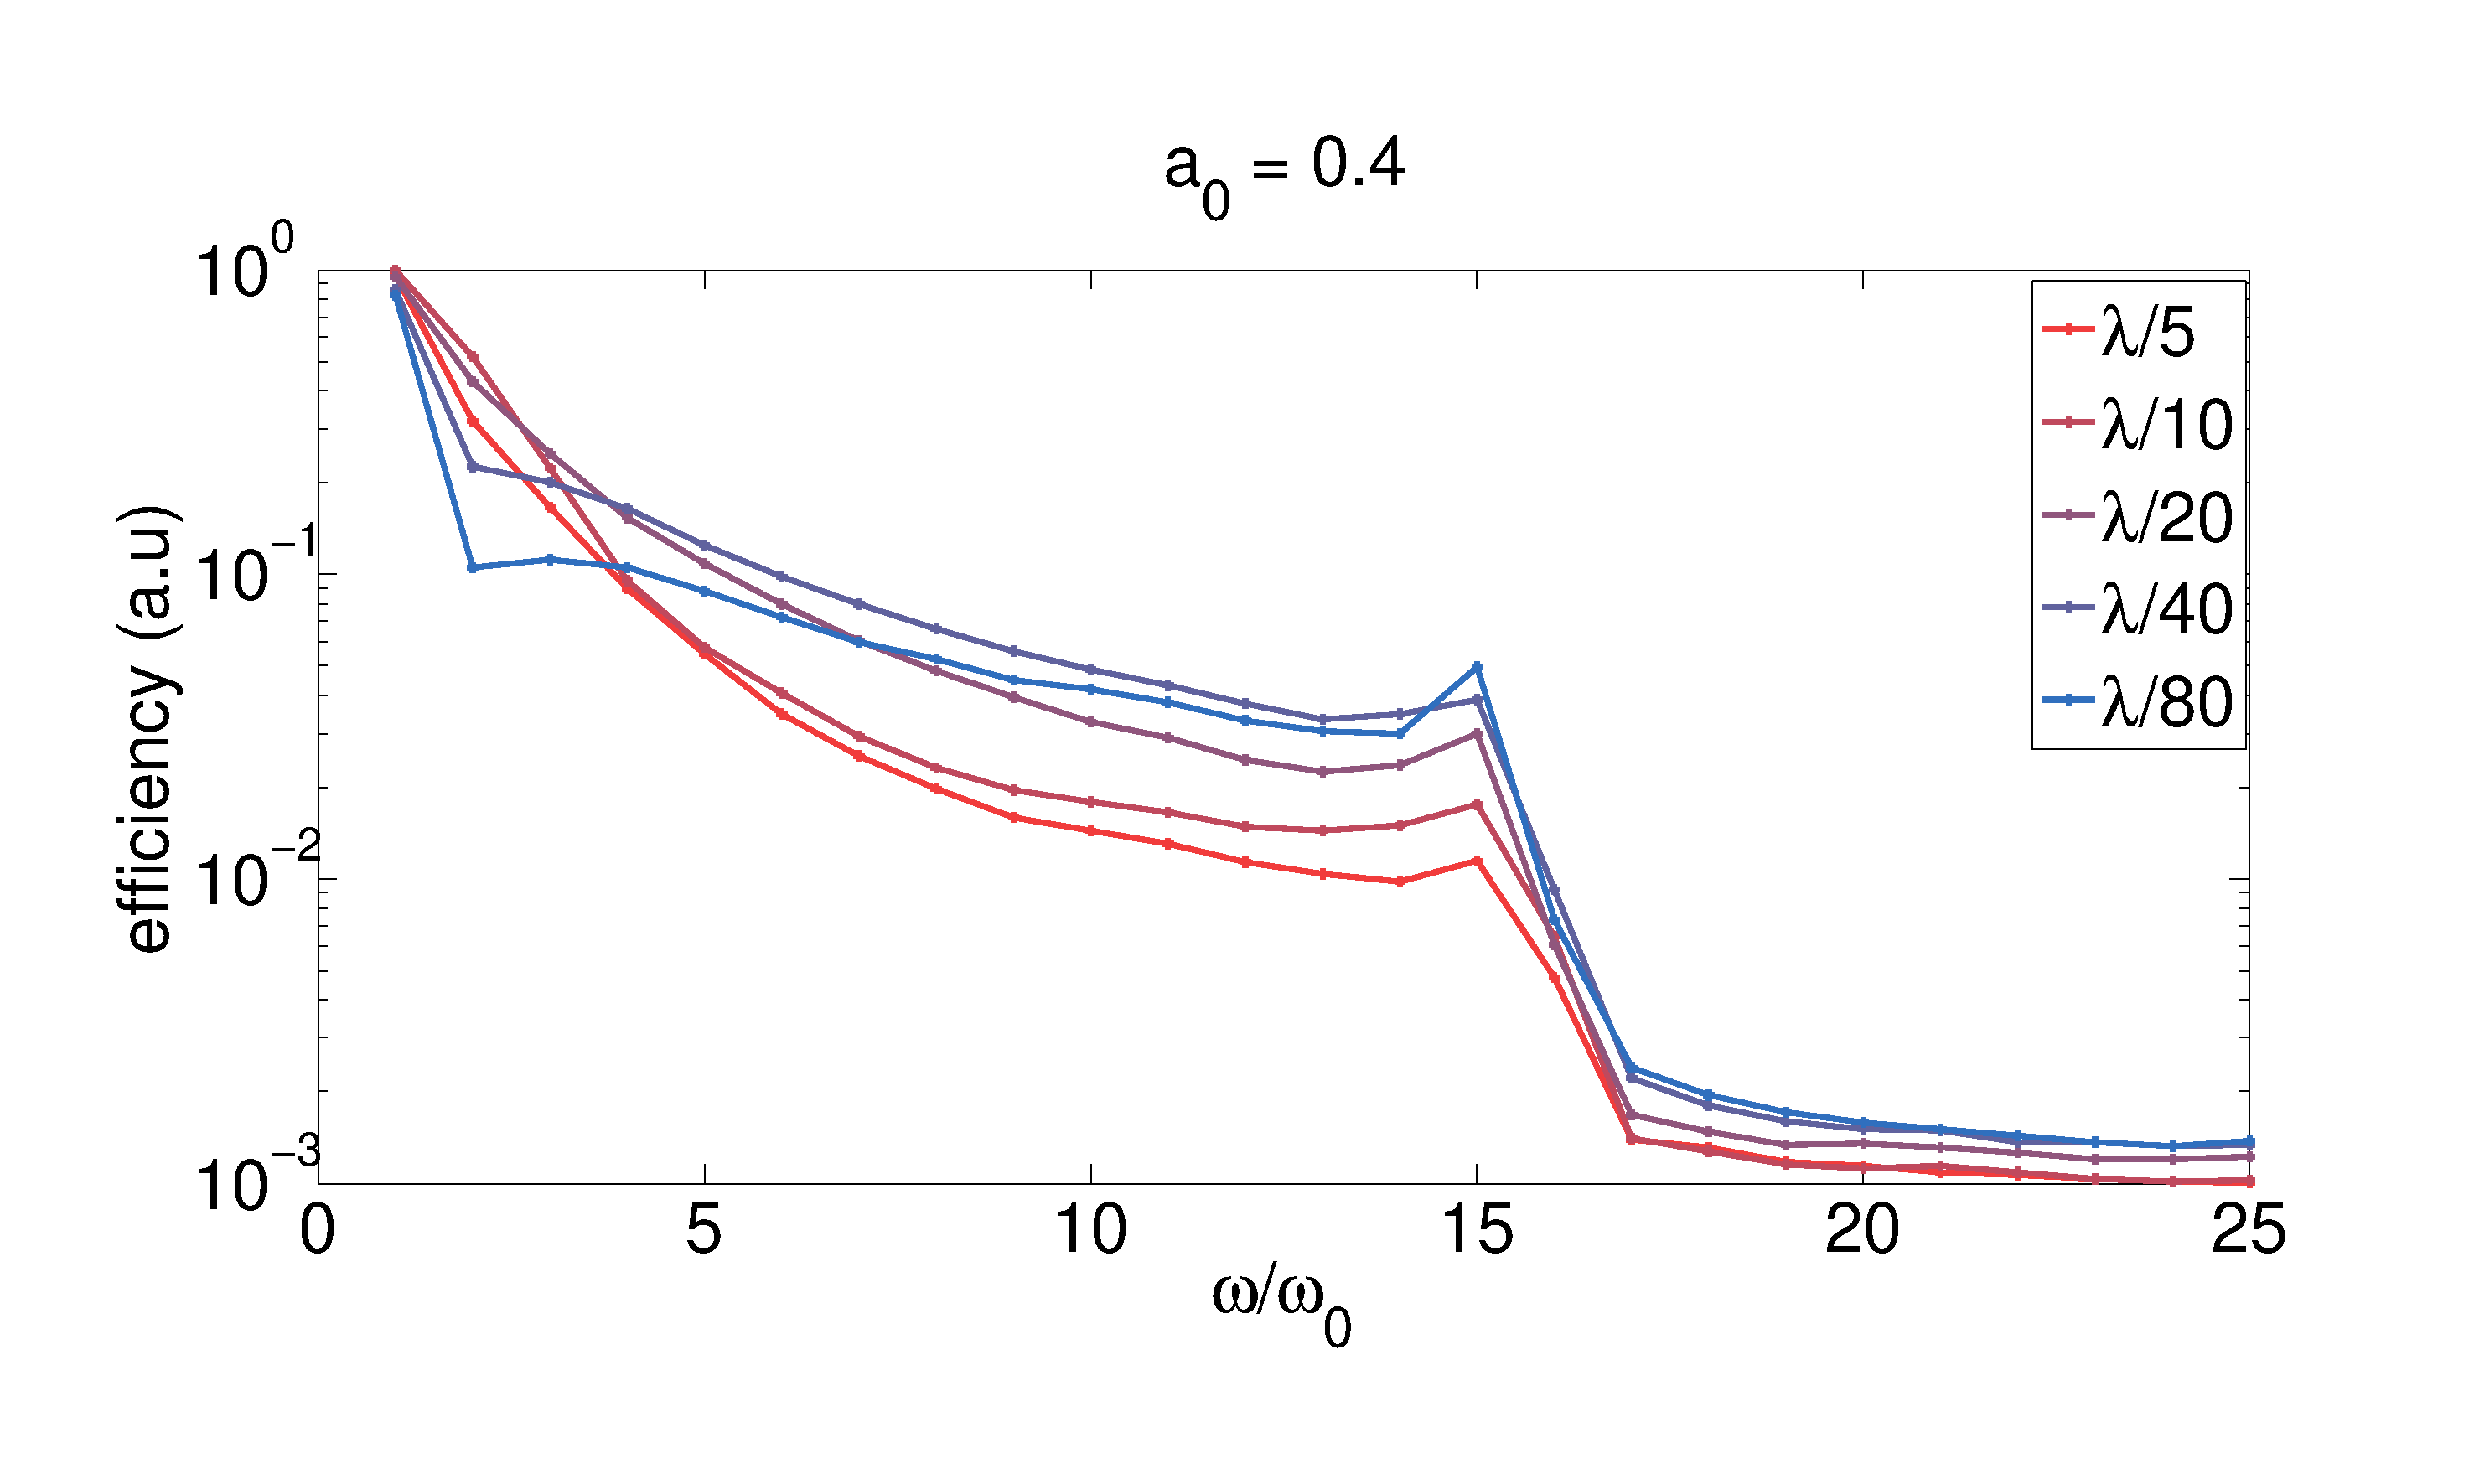
\includegraphics[width=\textwidth]{../chapitre6/images/a0=0p4.pdf}\\
\caption{\label{fig:a0=0p4}2D PIC simulation using Epoch: Influence of gradient length on CWE efficiency for $a_0 = 0.4$ and gradient scale lengths of respectively $L = \lambda/5, \lambda/10,\lambda/20,\lambda/40$ and $\lambda/80$. The peak at $\omega/\omega_0 = 15$ corresponds to a numerical resonance and is non-physical; the efficiency is plotted on a log scale.}
\end{figure}

\noindent In the simulation, the optimum appears for $L = \lambda/40$, that is to say for a gradient length nearly twice that observed in the experiment. This result is not surprising because  we estimated the expansion velocity to be $c_s\approx 6.8\,\mathrm{nm/ps}$ to convert the pump-probe delay to gradient length (the measuring technique is fully described in Chapter~\ref{ch:Measuring the gradient expansion}), but also made the hypothesis that the gradient length is rigorously equal to zero at time $t=0$.  It is important to note that when measuring the plasma expansion velocity over one laser wavelength, this assumption introduces a negligible error on the retrieved velocity provided the actual initial plasma scale length is negligible with respect to the laser wavelength. Here we see the initial plasma scale length should be on the order $\sim \lambda / 100$ for the experiment to fit the simulation.


\subsection{Reconstruction of harmonics in the far field}

We now consider the transverse dimension $y$ of the laser focus and calculate numerically the emission time over each point for a laser waist of $w_0 = 2.5\,\mathrm{\mu m}$ using the model presented in~\ref{subsection:CWE emission time}. This enables us to reconstruct a harmonic spectrogram with one coordinate being $y$ and the other the spectral frequency. Using a Fourier transform along $y$, the far field  harmonic spectrum is shown in Fig~\ref{fig:hhgfield_verticalspectral0}, where $\phi$ refers to the angular direction normal to the optical plane. 

\begin{figure}[H]
\centering
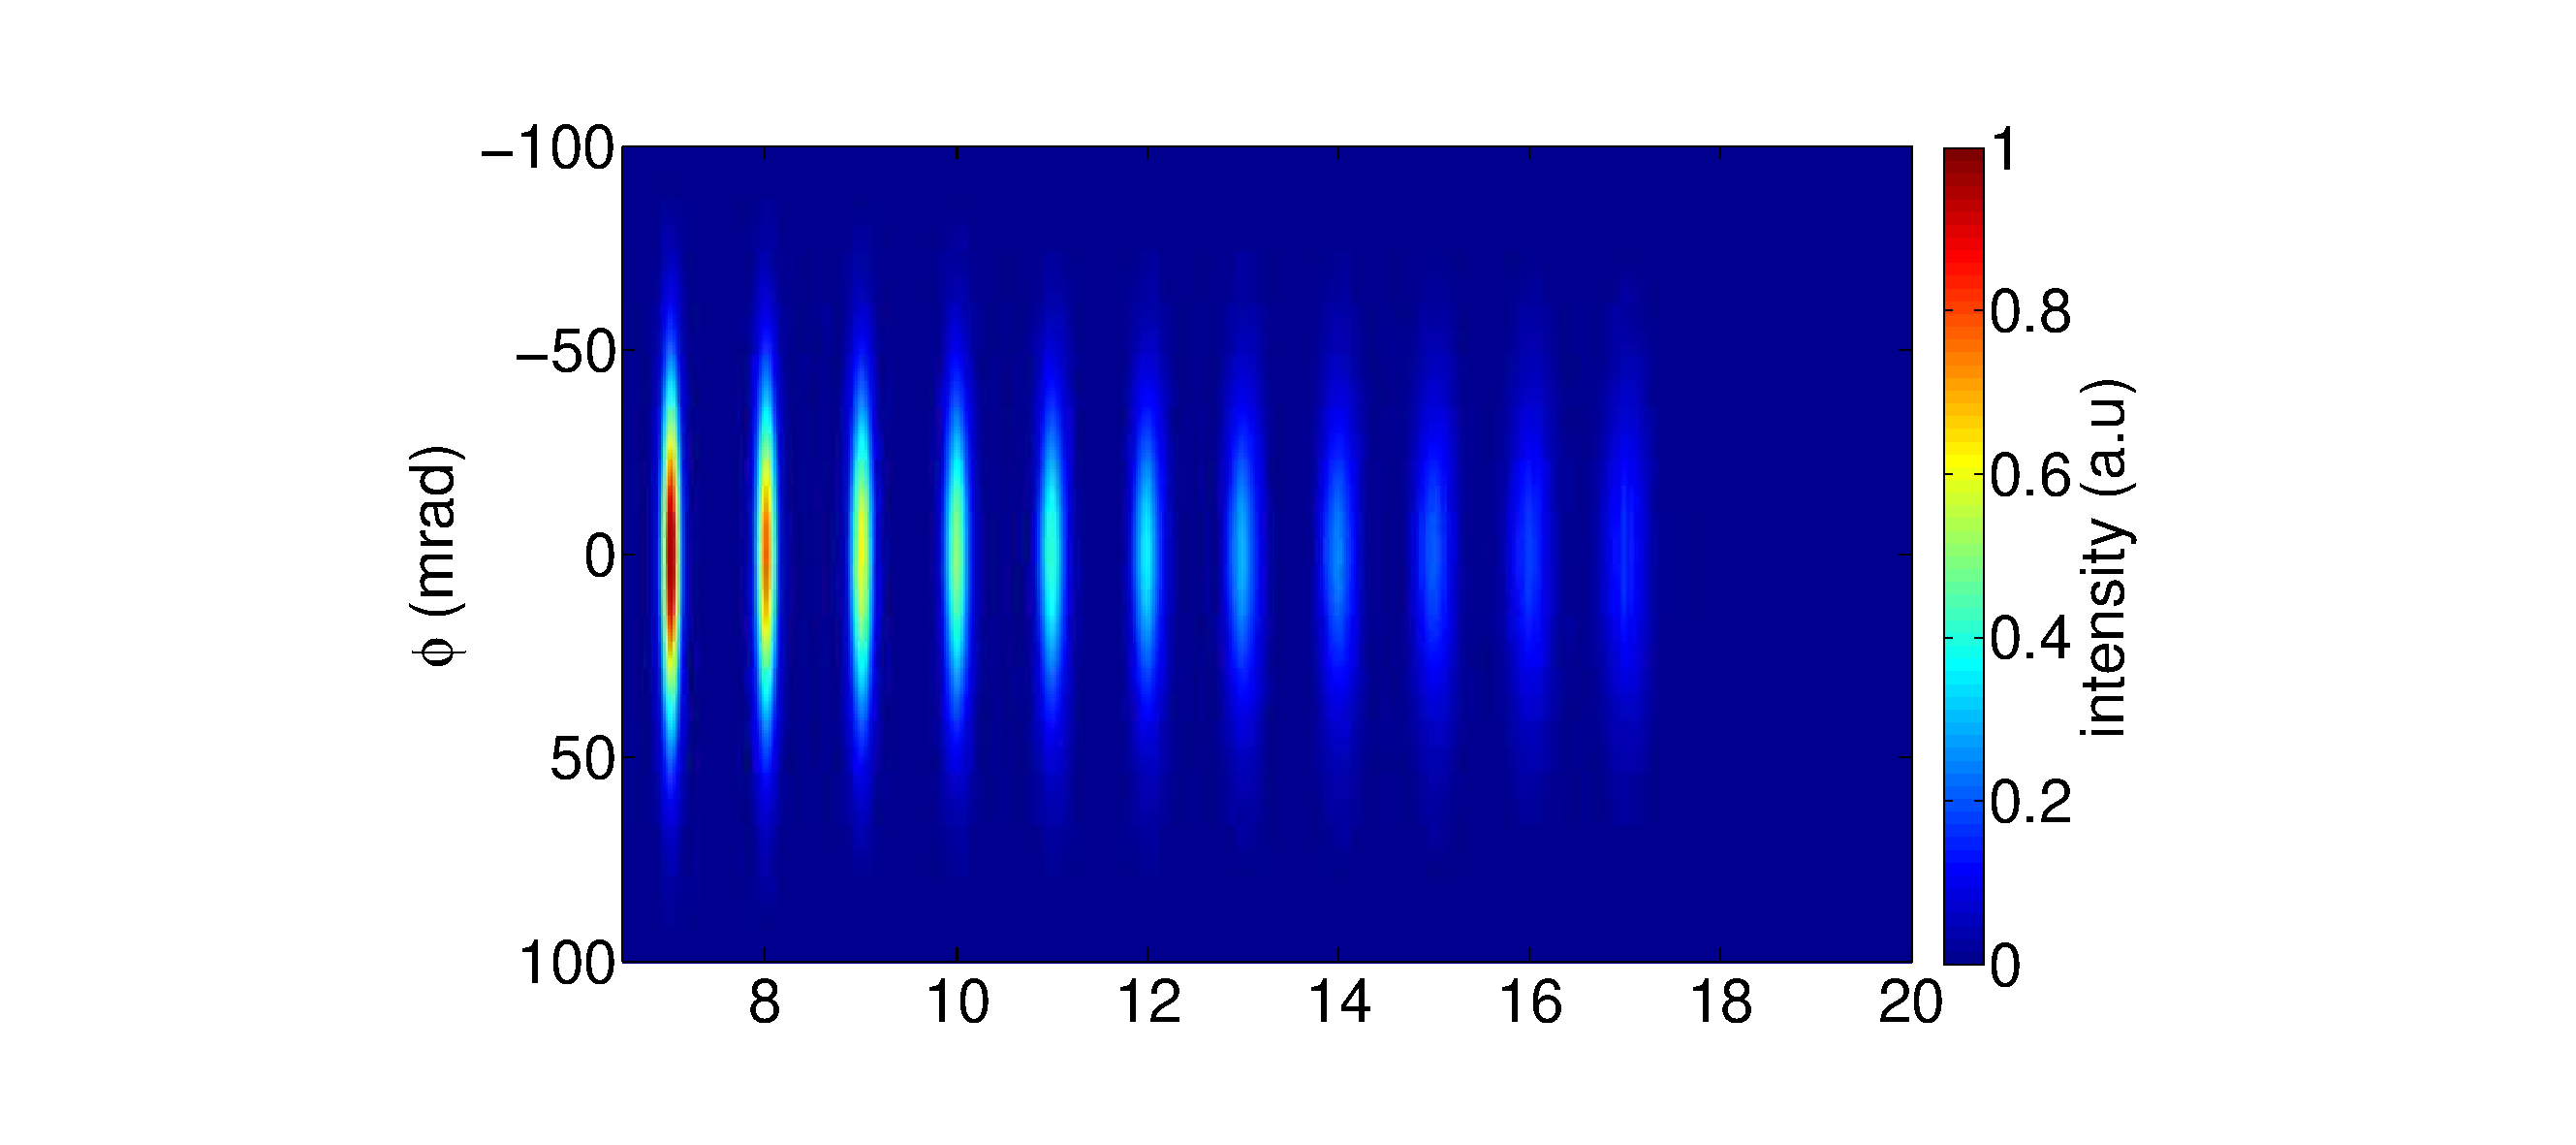
\includegraphics[width =\textwidth]{../chapitre6/images/hhgfield_verticalspectral.pdf}\\
\caption{\label{fig:hhgfield_verticalspectral0} Modelling of CWE emission spectra between H7 and H20 for a pulse of $30\,\mathrm{fs}$, a gradient length $L= \lambda / 100$ for laser intensity of $a_0 = 0.4$ and a waist $w_0=2.5\,\mathrm{\mu m}$}
\end{figure}

\noindent A representation of the temporal profile of the attosecond train is represented in Fig~\ref{fig:hhgfield_verticaltemporal}(a). In Fig~\ref{fig:hhgfield_verticaltemporal}(b), we zoom on one attosecond pulse taken between the two dotted white lines. This is a time-domain visualization of the spatial phase in the generation plane discussed in \ref{subsection:Harmonic spatial properties}.

\begin{figure}[H]
\centering
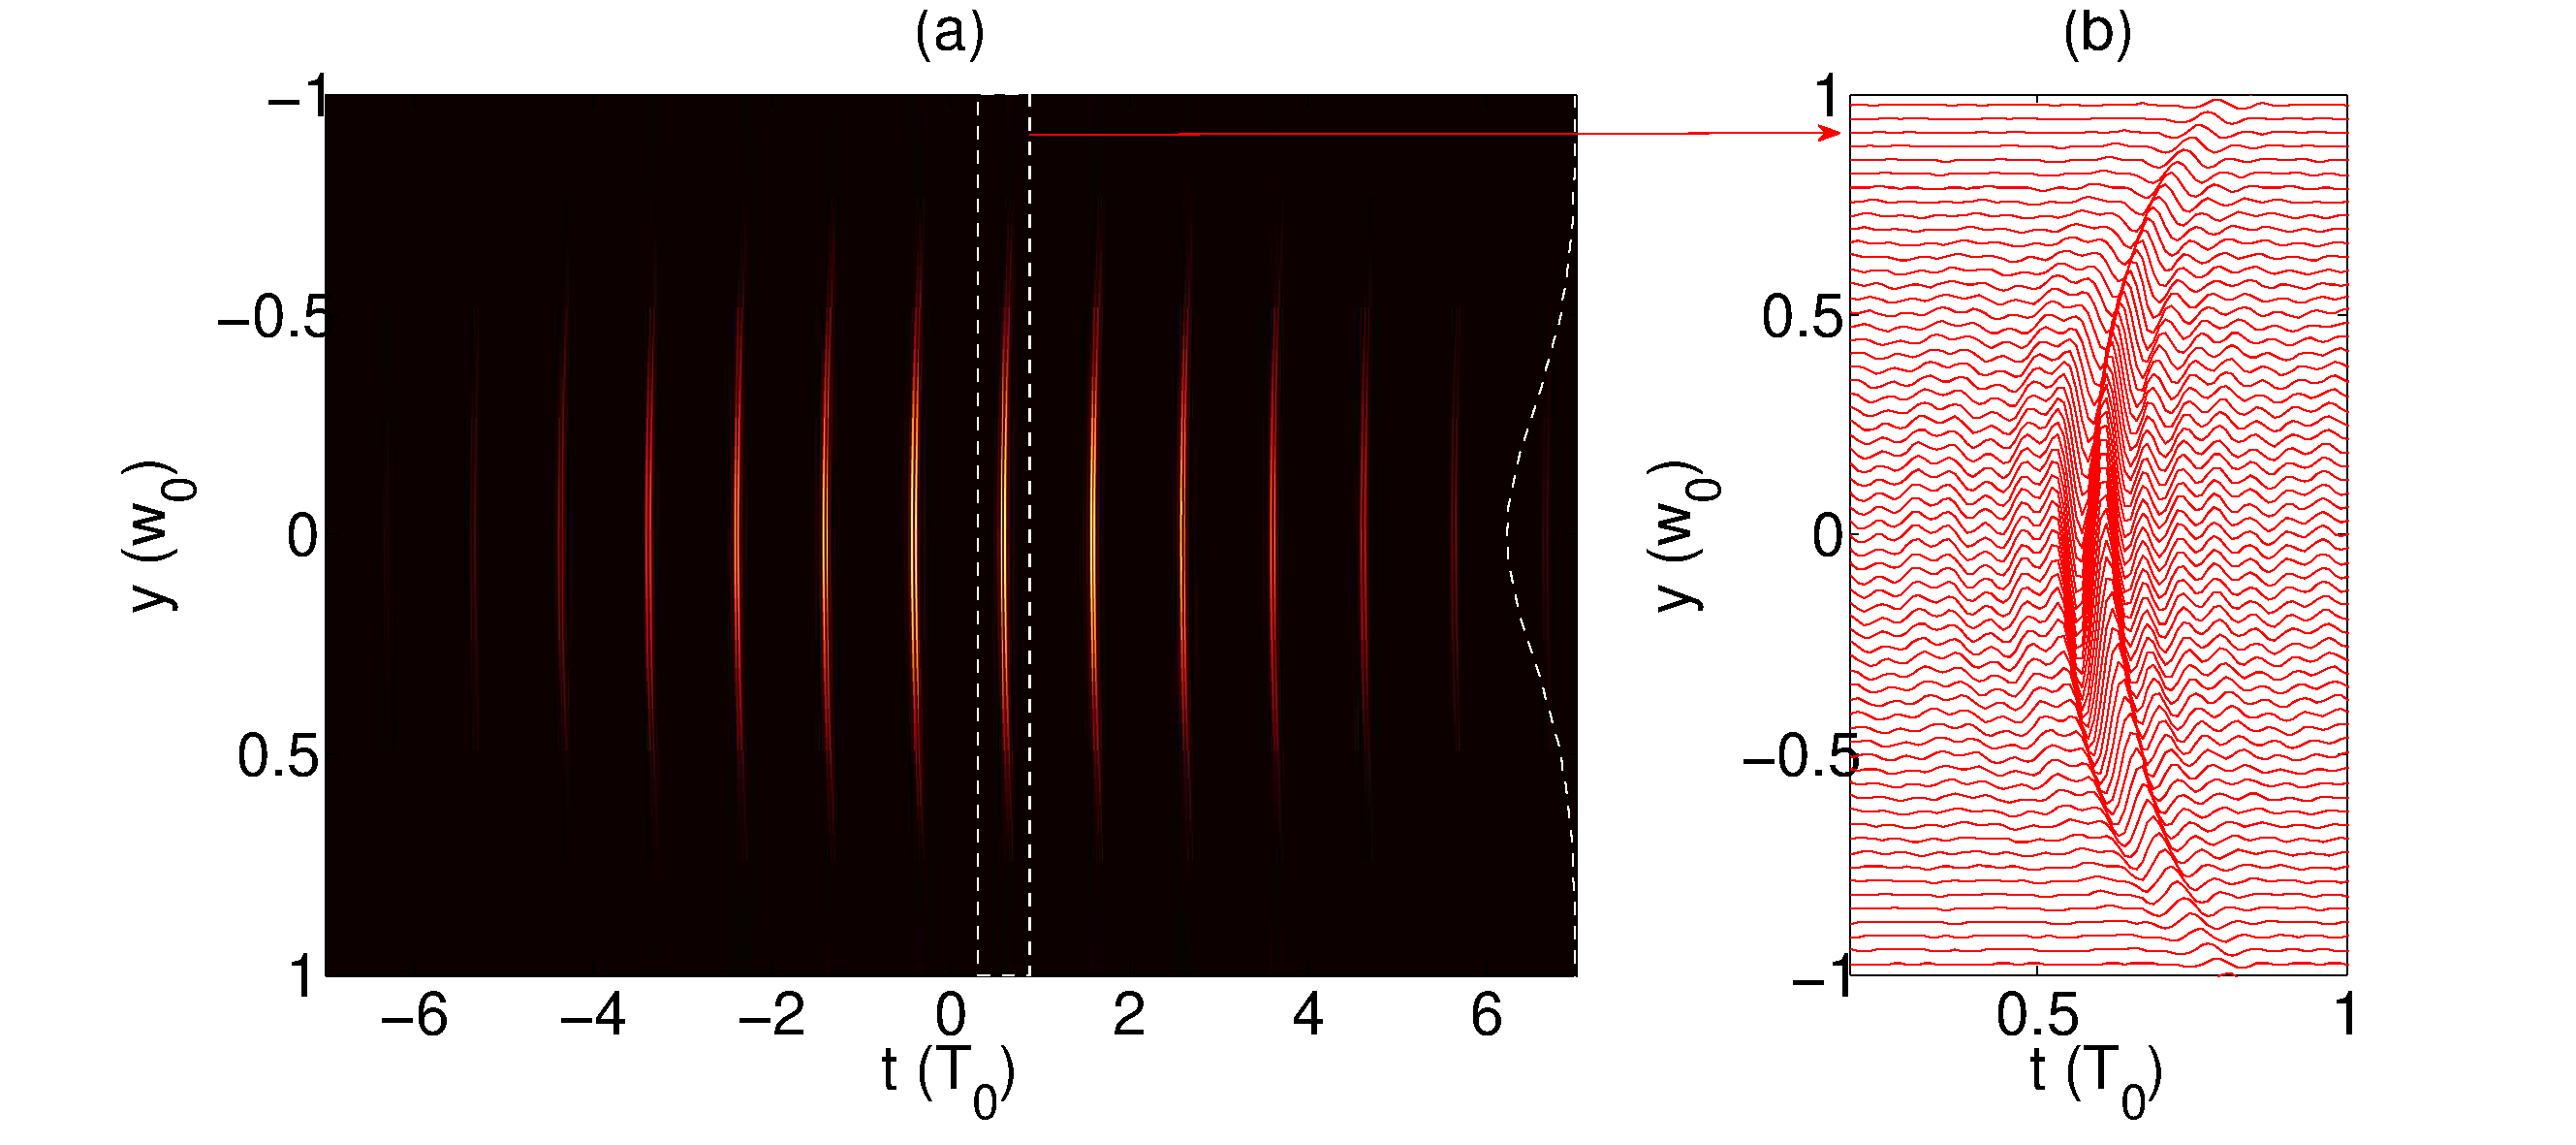
\includegraphics[width =\textwidth]{../chapitre6/images/hhgfield_verticaltemporal.pdf}\\
\caption{\label{fig:hhgfield_verticaltemporal} (a) CWE temporal emission along $y$ direction for a $30\,\mathrm{fs}$ Gaussian pulse, a gradient length $L= \lambda / 100$. The laser intensity of $a_0 = 0.4$ and its waist $w_0=2.5$. (b) Zoom on one attosecond pulse over one laser period.}
\end{figure}

\noindent The angular emission spectrum of an attosecond train, as we just explained, is intrinsically related to the spatially dependent emission time of each attosecond bunch. As a consequence, the laser spatio-temporal coupling (STC) will directly transfer to the harmonics~\cite{TheseHenri}. This simple statement naturally leads us to investigate the relative variation of spectrum and divergence with respect to a particular laser STC called Wavefront rotation, which we we describe in the following section.

\section{Attosecond chirp experiment}

\subsection{Definition of Wavefront rotation (WFR)}


Wavefront rotation (WFR) is a particular case of STCs~\cite{akturk2007first,akturk2006general}. In the presence of a spatial chirp at focus, the field can no longer be written as the product of a spatial profile times a temporal envelope, and the wavefronts can be viewed as "rotating" over time at velocity $v_{rot}$[mrad/fs]. The attosecond bunches resulting from the interaction are emitted in different directions of space. This so-called "attosecond lighthouse" was experimentally implemented in our group to generate isolated attosecond pulses \cite{theseAnto,Wheeler2012}, after it had been exposed by Henri Vincenti during his PhD~\cite{TheseHenri,vincenti2012attosecond}.\\

\noindent  When we misalign a dispersive element in the laser beam path, like a compressor grating or a pair of wedges, the $\vec{k}(\omega)$ vector of all spectral components $\omega$ are no longer collinear: the beam has an angular chirp, as represented in Fig~\ref{fig:WedgeWFR}. One can therefore directly derive the consequence for the beam at focus: each frequency will be focused at different position along the chirp direction such that the beam is said to be spatially chirped at focus.

\begin{figure}[H]
\centering
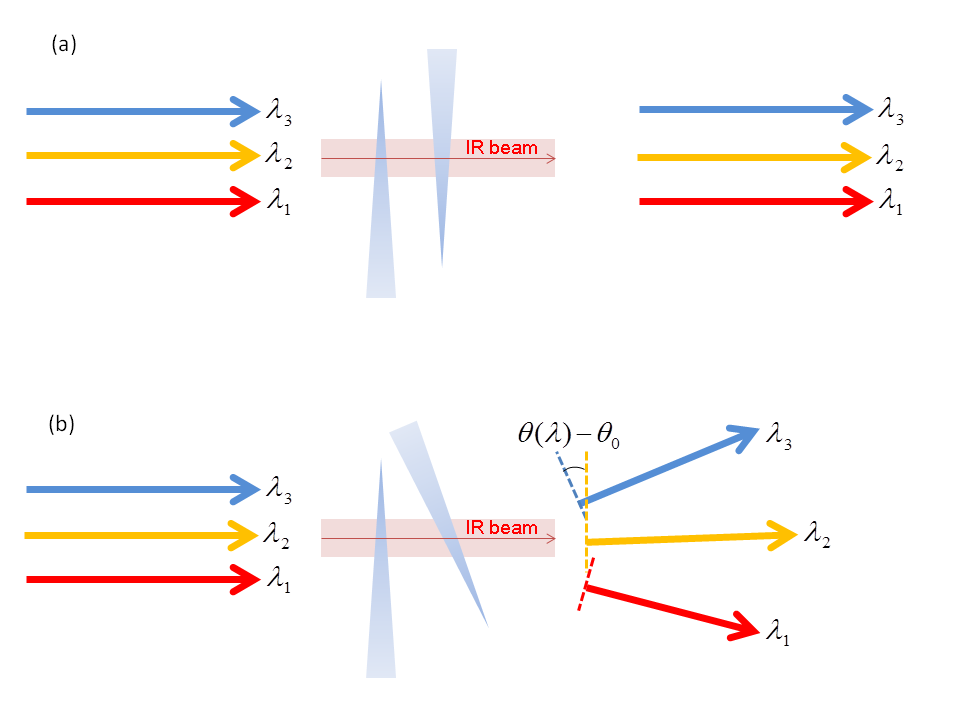
\includegraphics[width =\textwidth]{../chapitre6/images/WedgeWFR.png}\\
\caption{\label{fig:WedgeWFR} (a) Effect of propagation direction for different laser wavelengths when two wedges are parallel (b) One of the wedges is titled: the propagation direction for each wavelength is tilted by $\theta (\lambda) $ with respect to the initial case.}
\end{figure}

\noindent The influence of a spatial chirp at focus on the temporal profile of the pulse is illustrated in Fig~\ref{fig:WFRshema}. Looking only at the central line of the focal spot represented by a black dotted line, we illustrate how the temporal profile is distorted in presence of spatial chirp. In the $y>0$ region, the average frequency if blue shifted, which means the electric field period increases. On the contrary, towards the $y<0$ region, the average frequency is red shifted, which means the electric field period decreases. The result is that the beam wavefront appears to be rotating from cycle to cycle.

\begin{figure}[H]
\centering
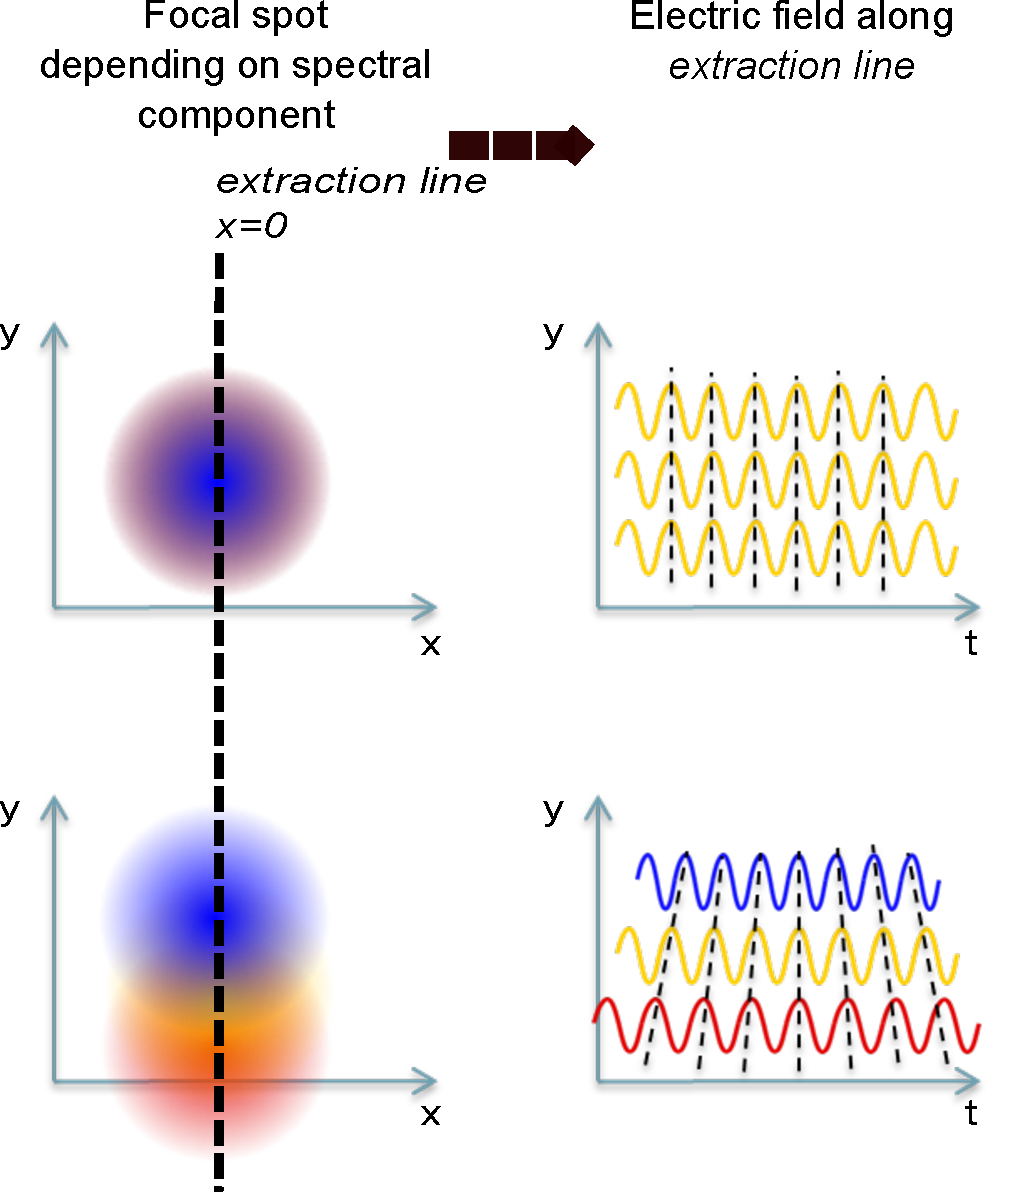
\includegraphics[width =0.5\textwidth]{../chapitre6/images/WFRshema.pdf}\\
\caption{\label{fig:WFRshema} Influence of spatial chirp at focus in artistic view. Top: no WFR when all wavelengths are spatially overlapped. Bottom: WFR because low frequencies are shifted towards the $y>0$ region and high frequencies towards the $y<0$ region.}
\end{figure}

\noindent The consequence of this effect is quite intuitive: from cycle to cycle, attosecond pulses are generated in a direction which "rotates" as a function of time.


\subsection{Analytical model to evaluate WFR at focus}
\label{subsub:Analytical model to evaluate WFR at focus}

We show here how we calculate the amount of WFR by only measuring the angular dispersion induced by the wedges (Fig~\ref{fig:WedgeWFR}). This simple model is compared to a measurement and is useful to calculate the emission time of the harmonics when the laser is spatially chirped at focus.\\

\noindent We call $\beta[\,\mathrm{\mu rad / nm}]$ the angular dispersion. The phase shift of each frequency along the vertical direction $y$ of the beam (the absolute reference $\phi =0$ is imposed for $\omega = \omega_0$ with no loss of generality) is given by:

\begin{equation}
\label{eq:defWFR}
\phi(y,\omega)[\mathrm{rad}] = k(\omega) y[\theta(\omega_0) + \int_{\omega}\beta(\lambda)d\lambda]=-k(\omega) y\int_{\omega}\beta(\omega)\frac{2\pi cd\omega}{\omega^2}
\end{equation}

\noindent We now only consider the first-order WFR  such that $\beta(\omega) = \beta$ is independent of $\omega$. An integration of Eq~\ref{eq:defWFR} leads to the expression:

\begin{equation}
\label{eq:defWFR2}
\phi(y,\omega)[\mathrm{rad}] = \alpha y
\end{equation}

\noindent where we define:
$$
\alpha[\,\mathrm{rad/mm}] = 2\pi\beta(1-\frac{\omega}{\omega_0})
$$



\noindent The expression of the collimated field $E_{\alpha,0}$ in the spectral domain with  WFR is simply related to the field before the wedges (which we write $E_{\alpha=0,0}$) by the product:

\begin{equation}
\label{eq:defWFR3}
E_{\alpha,0}(x,y,\omega) = E_{\alpha=0,0}(x,y,\omega)e^{i\alpha(\omega)y}
\end{equation}


\noindent We make the paraxial approximation such that the field with ($E_{\beta}$ ) or without ($E_{\beta=0}$ ) WFR at the focus of the parabola of focal length $f$ is written:

\begin{subequations}
\label{eq:defWFR4}
\begin{align}[left = \empheqlbrace\,]
     &E_{\beta=0}(x,y,\omega) = i\frac{\omega}{2 \pi f c}e^{-i\frac{\omega}{c}f}\mathscr{F}[E_{\alpha,0}](k_x = \frac{\omega x}{c f},k_y = \frac{\omega y}{c f}) \label{eq:eq:defWFR4-1}\\
     &E_{\beta}(x,y,\omega) = i\frac{\omega}{2 \pi f c}e^{-i\frac{\omega}{c}f}\mathscr{F}[E_{\alpha=0,0}](k_x = \frac{\omega x}{c f},k_y = \frac{\omega y}{c f})\label{eq:eq:defWFR4-2}
\end{align}
\end{subequations}



\noindent where $\mathscr{F}$ denotes the spatial 2D Fourier transform. Eq~\ref{eq:defWFR3} implies the simple relation~\cite{wefers1996space}:

\begin{equation}
\label{eq:defWFR5}
\mathscr{F}[E_{\alpha}](k_x,k_y,\omega)= \mathscr{F}[E_{\alpha=0}](k_x,k_y-\alpha(\omega),\omega)
\end{equation}

\noindent Combining Eq~\ref{eq:defWFR4} and Eq~\ref{eq:defWFR5}, we verify that adding WFR to a pulse is equivalent to shifting the focal spot center of wavelength $\lambda$ by a distance $\Delta y (\lambda)$:

\begin{equation}
E_{\beta}(x,y,\omega) = E_{\beta=0}(x,y-\Delta y (\omega),\omega)
\end{equation}

\noindent where:

 $$
\Delta y (\lambda)[mm] = 2\pi \beta f(\frac{1}{\omega}-\frac{1}{\omega_0})
$$

\noindent which gives after normalization by $\omega_0$:
$$
\overline{\Delta {y}} =  2\pi \beta  f (\frac{1}{\bar{\omega}}-1)
$$

\noindent Note that we have imposed the WFR to be equal to zero for $\bar{\omega} = 1$, meaning WFR is symmetric with respect to the carrier frequency $\omega_0$. 
In that case, we necessarily have $\overline{\Delta {y}} = 0$ for $\bar{\omega} = 1$. The different wavelengths therefore overlay at the center. By making a vertical transverse cut of the field at the position  $x = 0$ (just as done experimentally closing the entrance slit of our imaging spectrometer, described in ~\ref{subsub:Wavefront rotation measurement}), we find the expression for the field intensity
with ($\beta>0$) and without ($\beta=0$) WFR: 

\begin{equation}
S_{\beta = 0}(\omega,y) =  \omega^2 |E_{\beta=0}(0,\frac{\omega y}{c f},\omega)|^2
\end{equation}

\begin{equation}
S_{\beta}(\omega,y) =  \omega^2|E_{\beta = 0}(0,\frac{\omega (y- \Delta y(\omega))}{c f},\omega)|^2 = S_{\beta=0}(\omega,y-\Delta y (\omega))
\end{equation}

\noindent We can write that last relation using normalized variables for better clarity: 


\begin{equation}
\label{eq:RotationRelation}
S_{\beta = 0}(\bar{\omega},\bar{y}) =  S_{\beta=0}\left(\bar{\omega},\bar{y}-2\pi  \beta  f (\frac{1}{\bar{\omega}}-1)\right)
\end{equation}



\noindent Based on Eq~\ref{eq:RotationRelation}, we can construct a simple geometrical transformation to emulate the intensity shaping resulting from WFR at focus. In particular, posing $X = \frac{1}{\bar{\omega}}$ et $Y = \bar{y}$. We define the function $\hat{S}$ of natural variables $X,Y$ by the relation:

\begin{equation}
  \left\{
      \begin{aligned}
        &\hat{S}_{\beta=0}(X,Y) = S_{\beta = 0}(\frac{1}{X},Y) \\
        &\hat{S}_{\beta}(X,Y) = S_{\beta}(\frac{1}{X},Y) = S_{\beta=0}(\frac{1}{X},Y-2\pi\beta f (X-1)) = \hat{S}_{\beta=0}(X,Y-2\pi\beta f(X-1))  \\
      \end{aligned}
    \right.
\end{equation}


\noindent We now see that  $\hat{S}_{\beta}$ et $\hat{S}_{\beta=0}$ are simply related by linear transformation of the system of coordinates:

$$
\left( \begin{array}{c}
X'\\
Y'\end{array} \right)=
\left( \begin{array}{cc}
1&0\\
-2\pi f\beta &1\end{array} \right)\left( \begin{array}{c}
X \\
Y \end{array} \right)+\left( \begin{array}{c}
0\\
2\pi f\beta \end{array} \right)
$$

\noindent where we clearly identify a shearing of the coordinates $X$, $Y$.

\subsection{WFR measurement}\label{subsub:Wavefront rotation measurement}

The experimental setup allowing us to control the angular chirp  of the main laser pulse is represented in Fig~\ref{fig:SETUP_hhg_wedges}. Wedges are introduced in the main beam path at Brewster angle in a parallel configuration. WFR in the plane of polarization is obtained by turning one of the wedges with respect to the other. For the WFR to be in the vertical plane, we introduce a periscope after the wedges, which rotate the WFR direction, but unfortunately also the beam polarization as indicated in Fig~\ref{fig:SETUP_hhg_wedges}. Therefore, we add a half-wave plane after the periscope. This way, the polarization is turned back to P with respect to the target while the WFR remains vertical.

\begin{figure}[H]
\centering
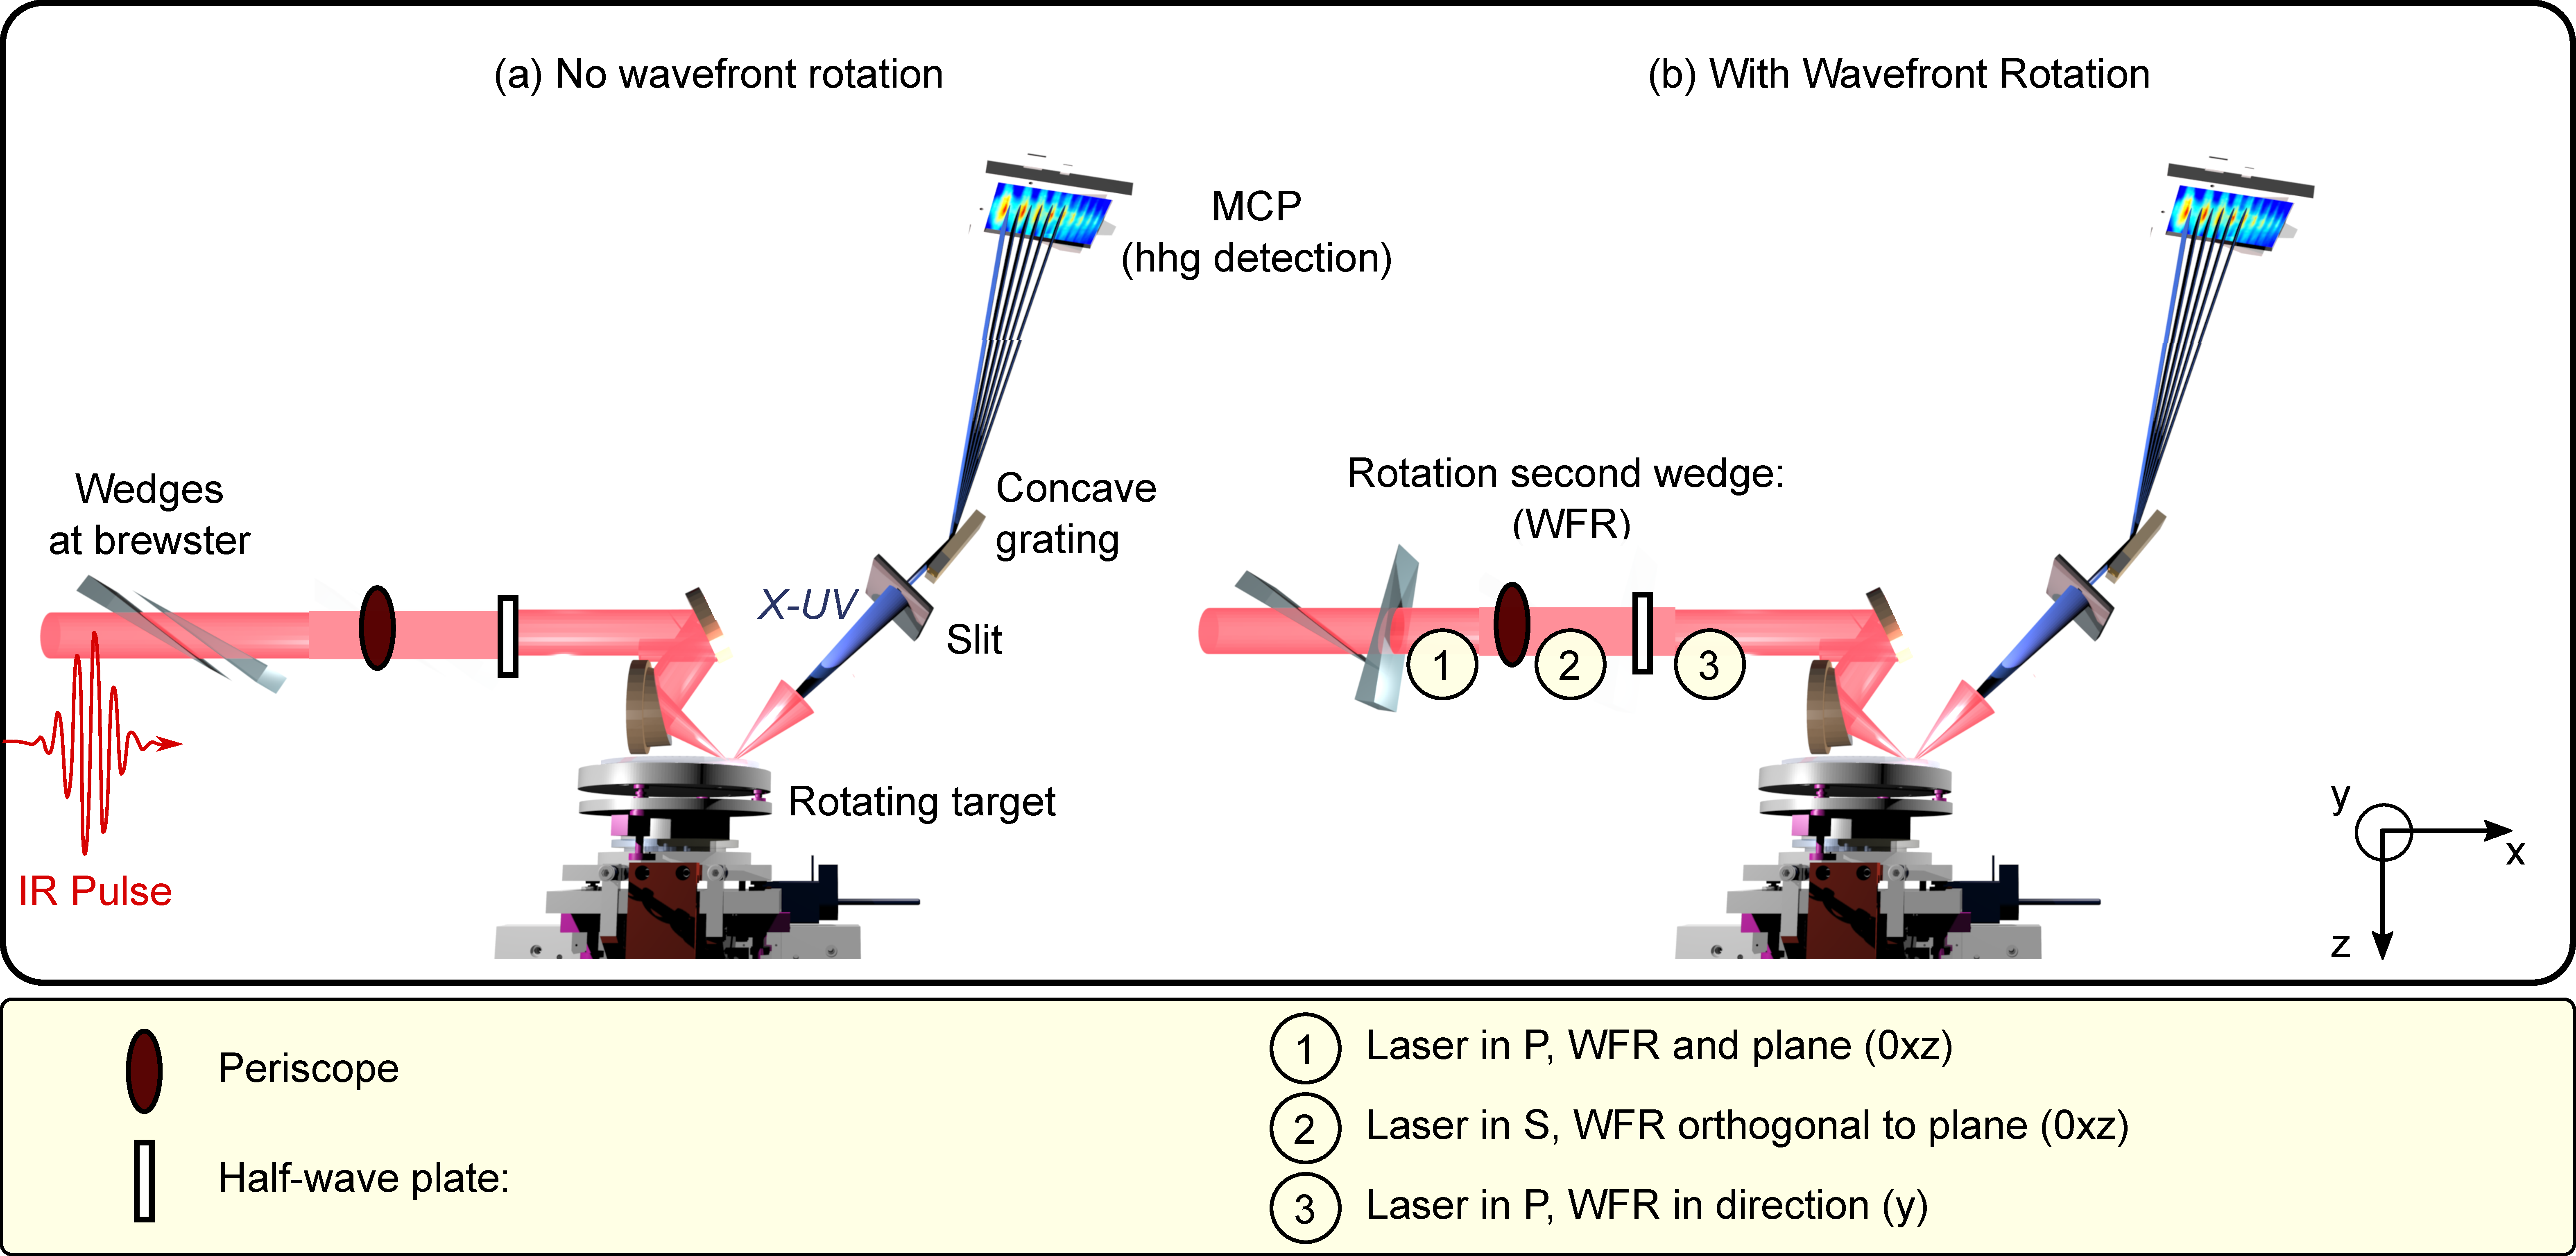
\includegraphics[width =\textwidth]{../chapitre6/images/SETUP_hhg_wedges.pdf}\\
\caption{\label{fig:SETUP_hhg_wedges} Experimental setup: Wedges are introduced in the main beam path in a parallel configuration (a). WFR is obtained by turning one of the wedges with respect to the other (b)}
\end{figure}

\noindent WFR can be measured by imaging the focal spot of the laser on the entrance slit of an imaging spectrometer.



\begin{figure}[H]
\begin{center}
\makebox[\textwidth][c]{
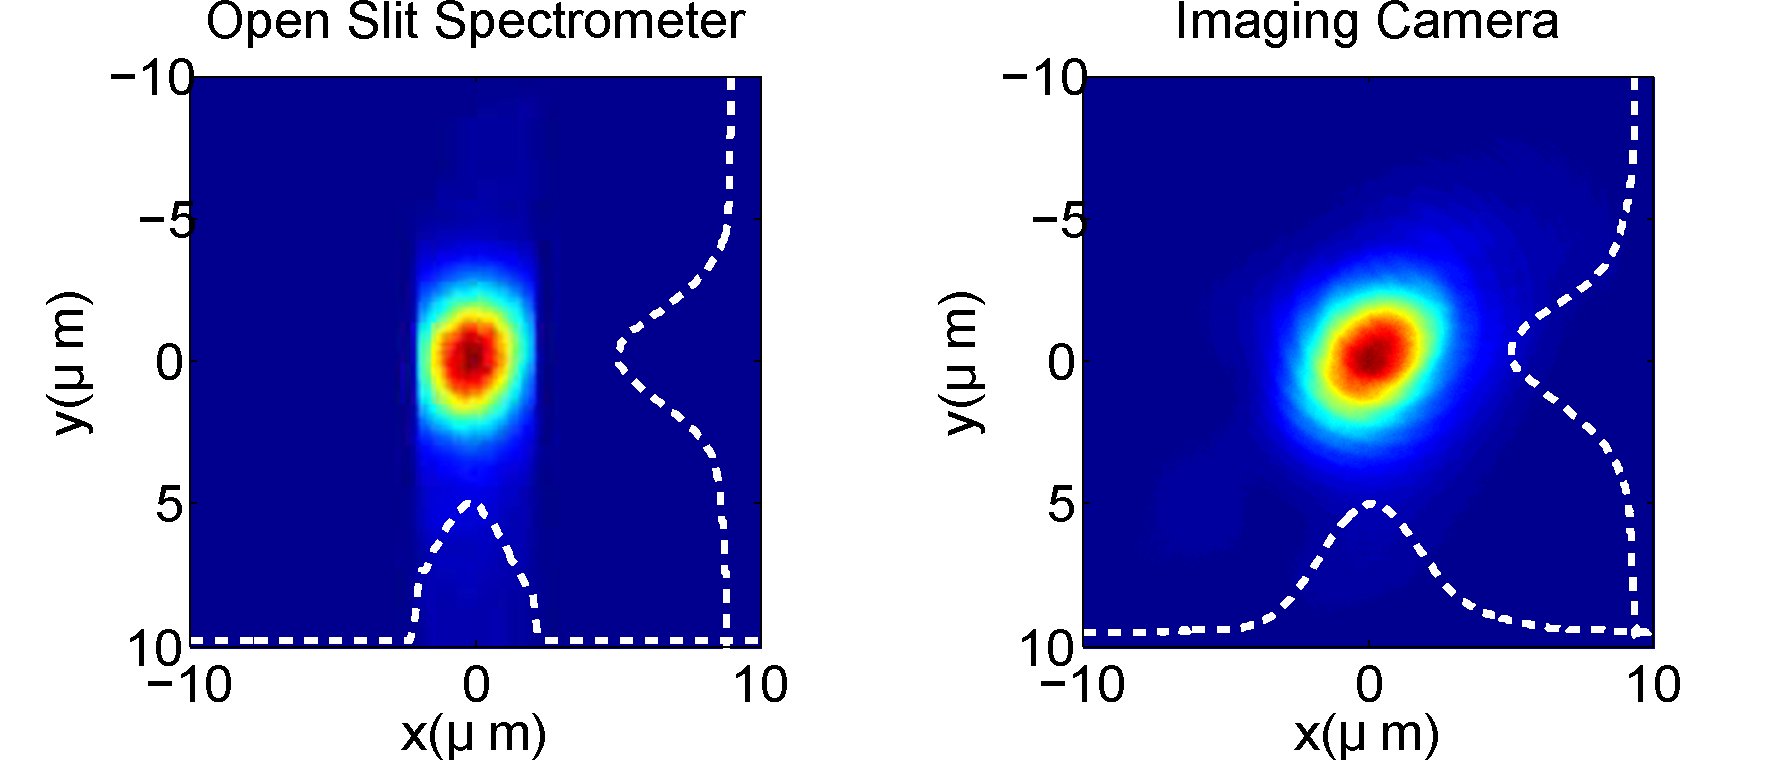
\includegraphics[width =\textwidth]{../chapitre6/images/Focal_20140806_calibration.pdf}}\\
\caption{\label{Focal_20140806_calibration} Imaging spectrometer at $0^{th}$ order with an open slit (left) after setting the calibration $0.09\,\mathrm{\mu m / px}$. The measured focal spot is $4\,\mathrm{\mu m}$ (FWHM). Comparison to an image given by our standard imaging camera (right)}
\end{center}
\end{figure}



\noindent  By closing this slit to let through the light in the central vertical line of the spot
and adjusting the diffraction grating to the central wavelength ($800\,\mathrm{nm}$), we can retrieve the spectrum at each position $y$ of the focus. Fig~\ref{Focal_20140806_calibration} shows the profile of the focal spot imaged on the open slit (right) when the grating is positioned to reflect the $0^{th}$ order (i.e. specular reflection), where we find the focus to be $4\,\mathrm{\mu m}$ at FWHM.
We now apply this transformation described in~\ref{subsub:Analytical model to evaluate WFR at focus} to a temporal and spatial Gaussian beam with $\tau_{fwhm} = 30 \mathrm{fs}$.
The angular dispersion $\beta$ is calculated theoretically from the relative angle of the two prisms, and reported in the following table:\\

\begin{center}
\begin{tabular}{c|c|c|c|c|c|c|c}
\hline
\hline
angle(deg) &70&60&50&40&30&15&0\\
\hline
$\beta$($\mu$ rad/nm)&2.012&0.9049&0.4799&0.2545&0.1232&0.02369&0\\
\hline
\hline
\end{tabular}
\end{center}


\begin{figure}[H]
\makebox[\textwidth][c]{
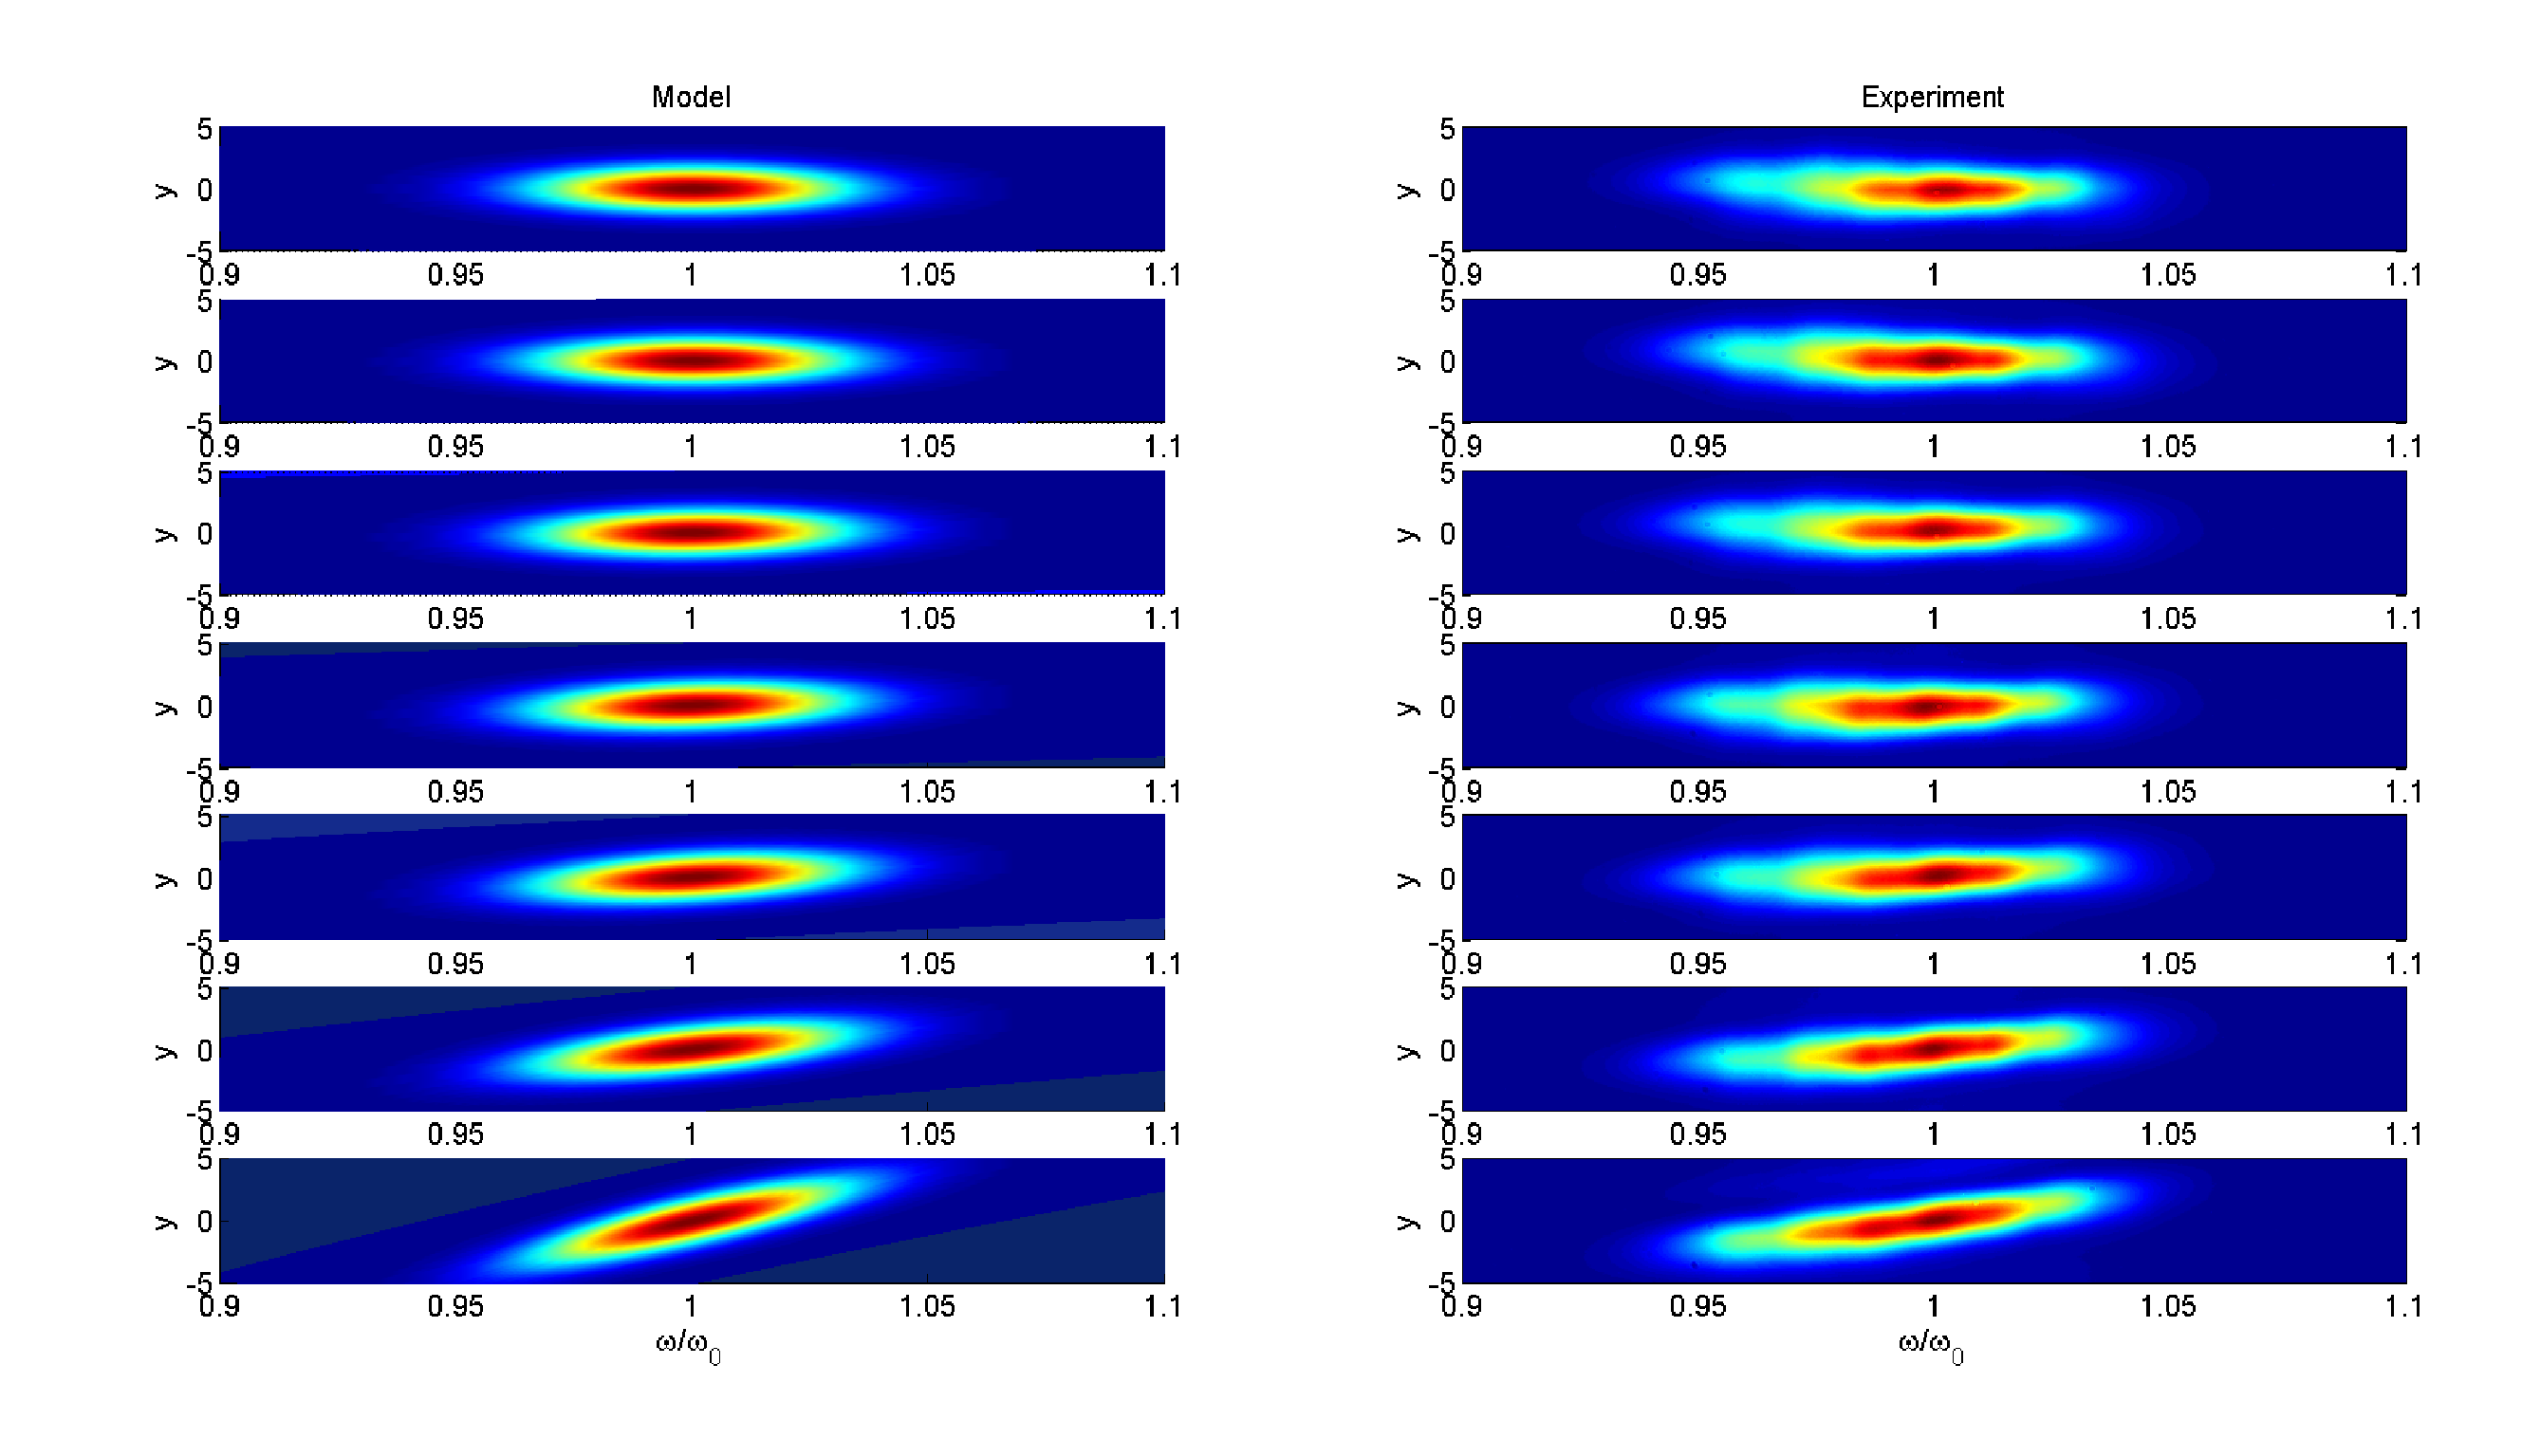
\includegraphics[width =1.1\textwidth, height = 10cm]{../chapitre6/images/SimulationWFR-focus2p5um.pdf}}
\caption{\label{fig:SchemaFrogAtto} Comparison of model to experimental measurement of vertically resolved pulse spectra with WFR at focus, where y is given in $\,\mathrm{\mu m}$. In the model (left) we considered a $30\,\mathrm{fs}$ pulse with the spatial dimension as measured experimentally. The spectra $S(\omega,y)$ is obtained by shearing the coordinate as described in \ref{subsub:Analytical model to evaluate WFR at focus}. The experimental measured spectra are obtained by rotating the wedges of $\theta =$0° (top), 15°, 30°, 40°, 50°, 60° and 70° (bottom) in order. }
\end{figure}

\noindent One can then calculate the WFR velocity by calculating the variation of the mean frequency along $y$, which leads to Fig~\ref{fig:Vrot}. For a given spectrum, the wavefront rotation does not always increase with the angular dispersion (or the angle of the wedge). There exists an optimal value. This is understandable because as the spatial chirp increases at focus, the beam ``elongates'' which has the effect of decreasing the WFR. The optimal angle for the wedges is a trade-off between the spectral spread of the different frequencies along $y$ with which $V_{rot}$ increases and the beam spatial elongation with which $V_{rot}$ decreases. The existence of such an optimum has been studied in great detail in \cite{TheseHenri} and is clearly  visible in Fig~\ref{fig:Vrot}. 



\begin{figure}[H]
\centering
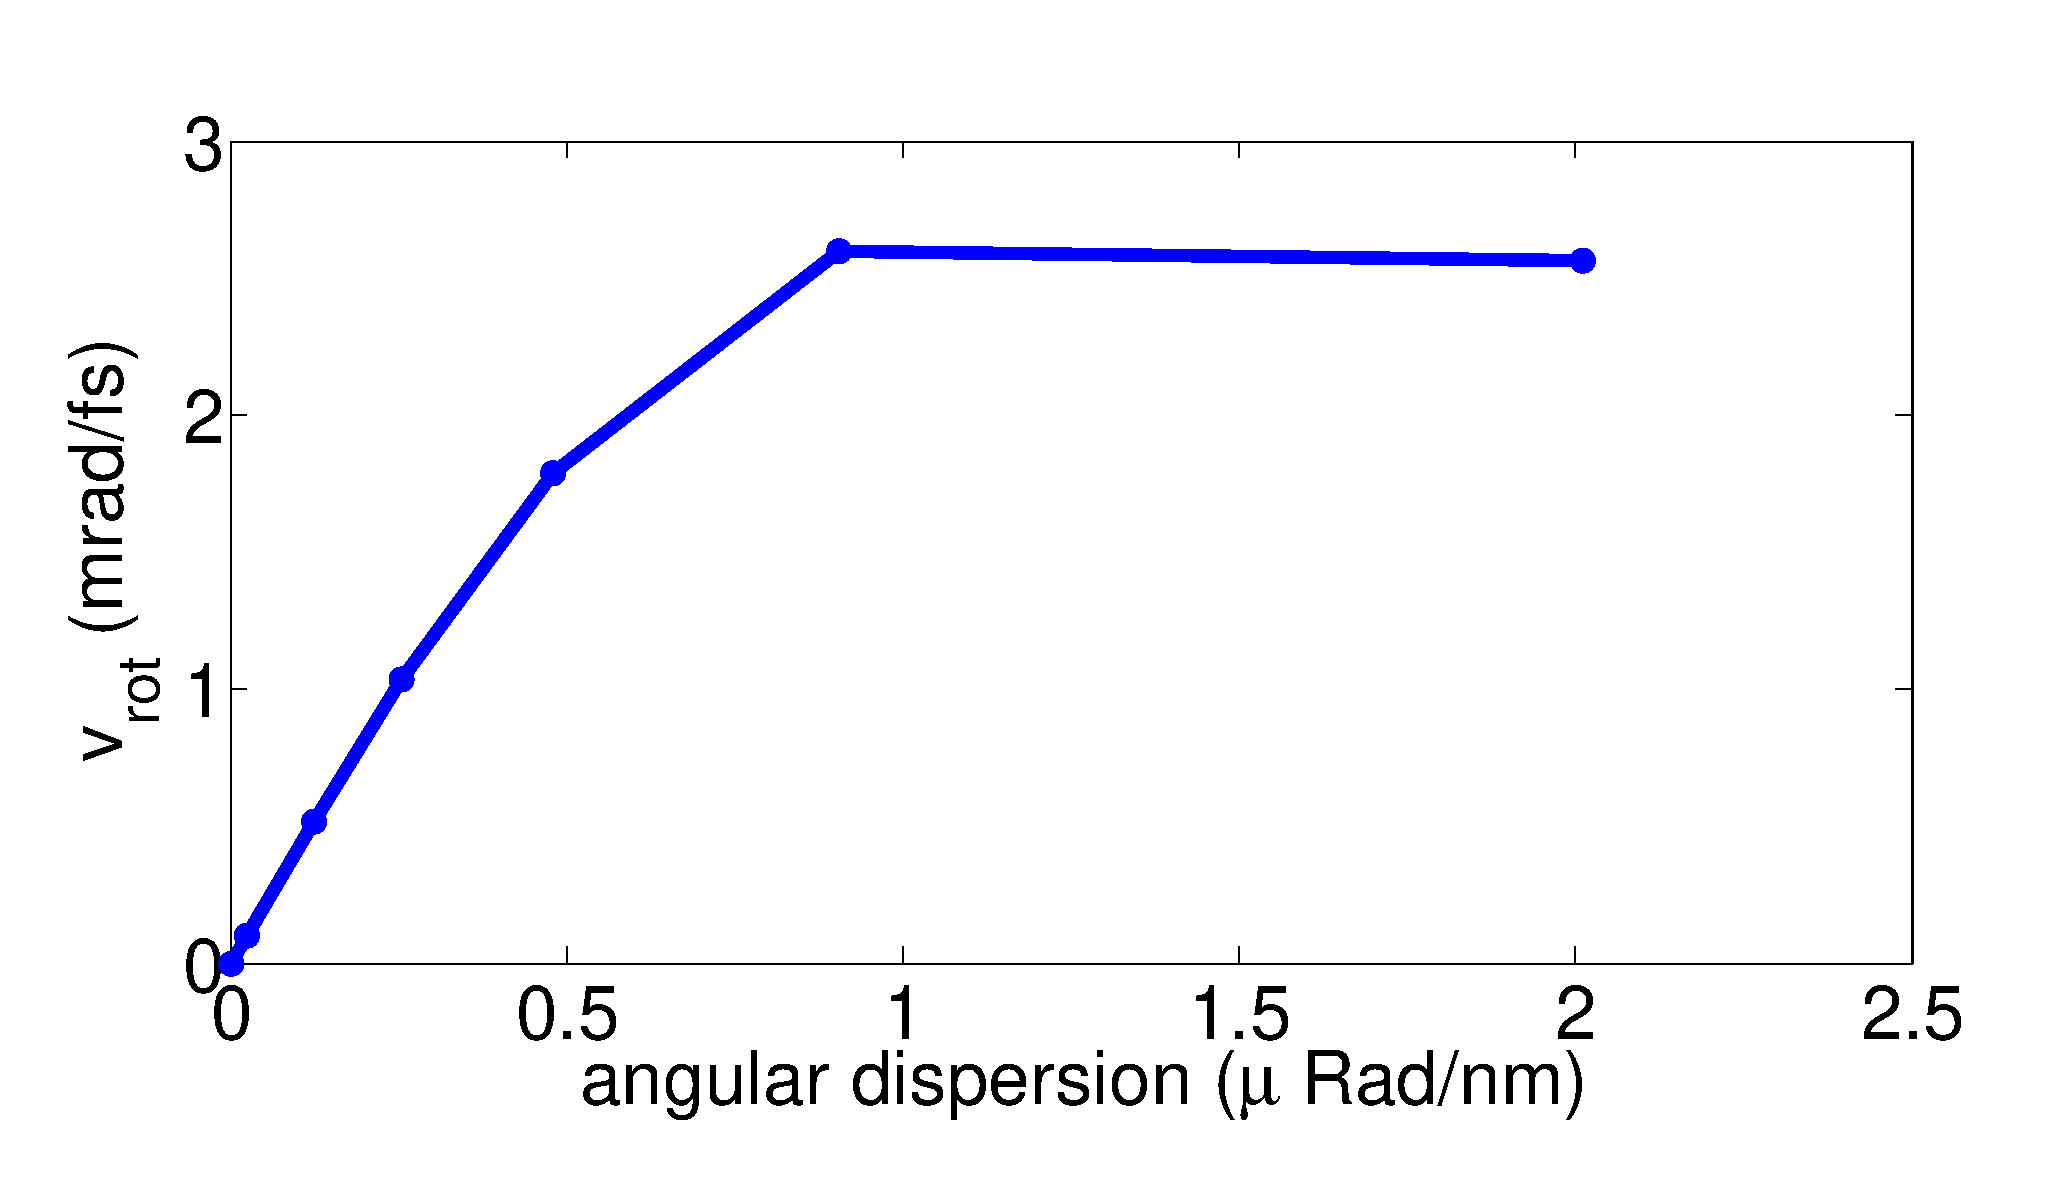
\includegraphics[width =0.9\textwidth]{../chapitre6/images/Vrot.pdf}\\
\caption{\label{fig:Vrot} Evaluation of $V_{rot}$ with respect to angular dispersion $\beta$ calculated for each angular position of the wedges using the analytical model described in \ref{subsub:Analytical model to evaluate WFR at focus} }
\end{figure}

\noindent \g{Effect of WFR on harmonic generation:}\\
\noindent Fig~\ref{fig:hhgfield_verticalspectral} presents a comparison between the simulation using the 1D model and the experimental measurement of the angularly-resolved spectrum harmonics (H7 to H17) when WFR is added at the focus by rotating the second wedge by $70^{\circ}$. The first observation is that both in the model and the experiment, the harmonics are tilted when WFR is added to the driving laser at focus. This effect was predicted, because as we described in \ref{subsection:CWE emission time}, the periodicity of the attosecond train increases during the generation process. But since in the presence of WFR, the beginning of the pulse is emitted in the direction of high angles, and the end in the direction of low angles, the recorded image on the MCP is the result of a time-to-space mapping of the attosecond pulses. Because of this, the upper region of the spectrum will be blue shifted while the lower one will be red shifted, i.e. the harmonics become ``tilted''. In the experiment, we note that in the absence of WFR, the harmonics are spectrally wider than in the model, which indicates an undervaluation of the femtosecond chirp in the model. A second observation is that the tilt in presence of WFR is more pronounced in the experiment, which again is symptomatic of strong femtosecond chirp and therefore consistent with the broad harmonic line profile observed in the absence of WFR. 


\begin{figure}[H]
\centering
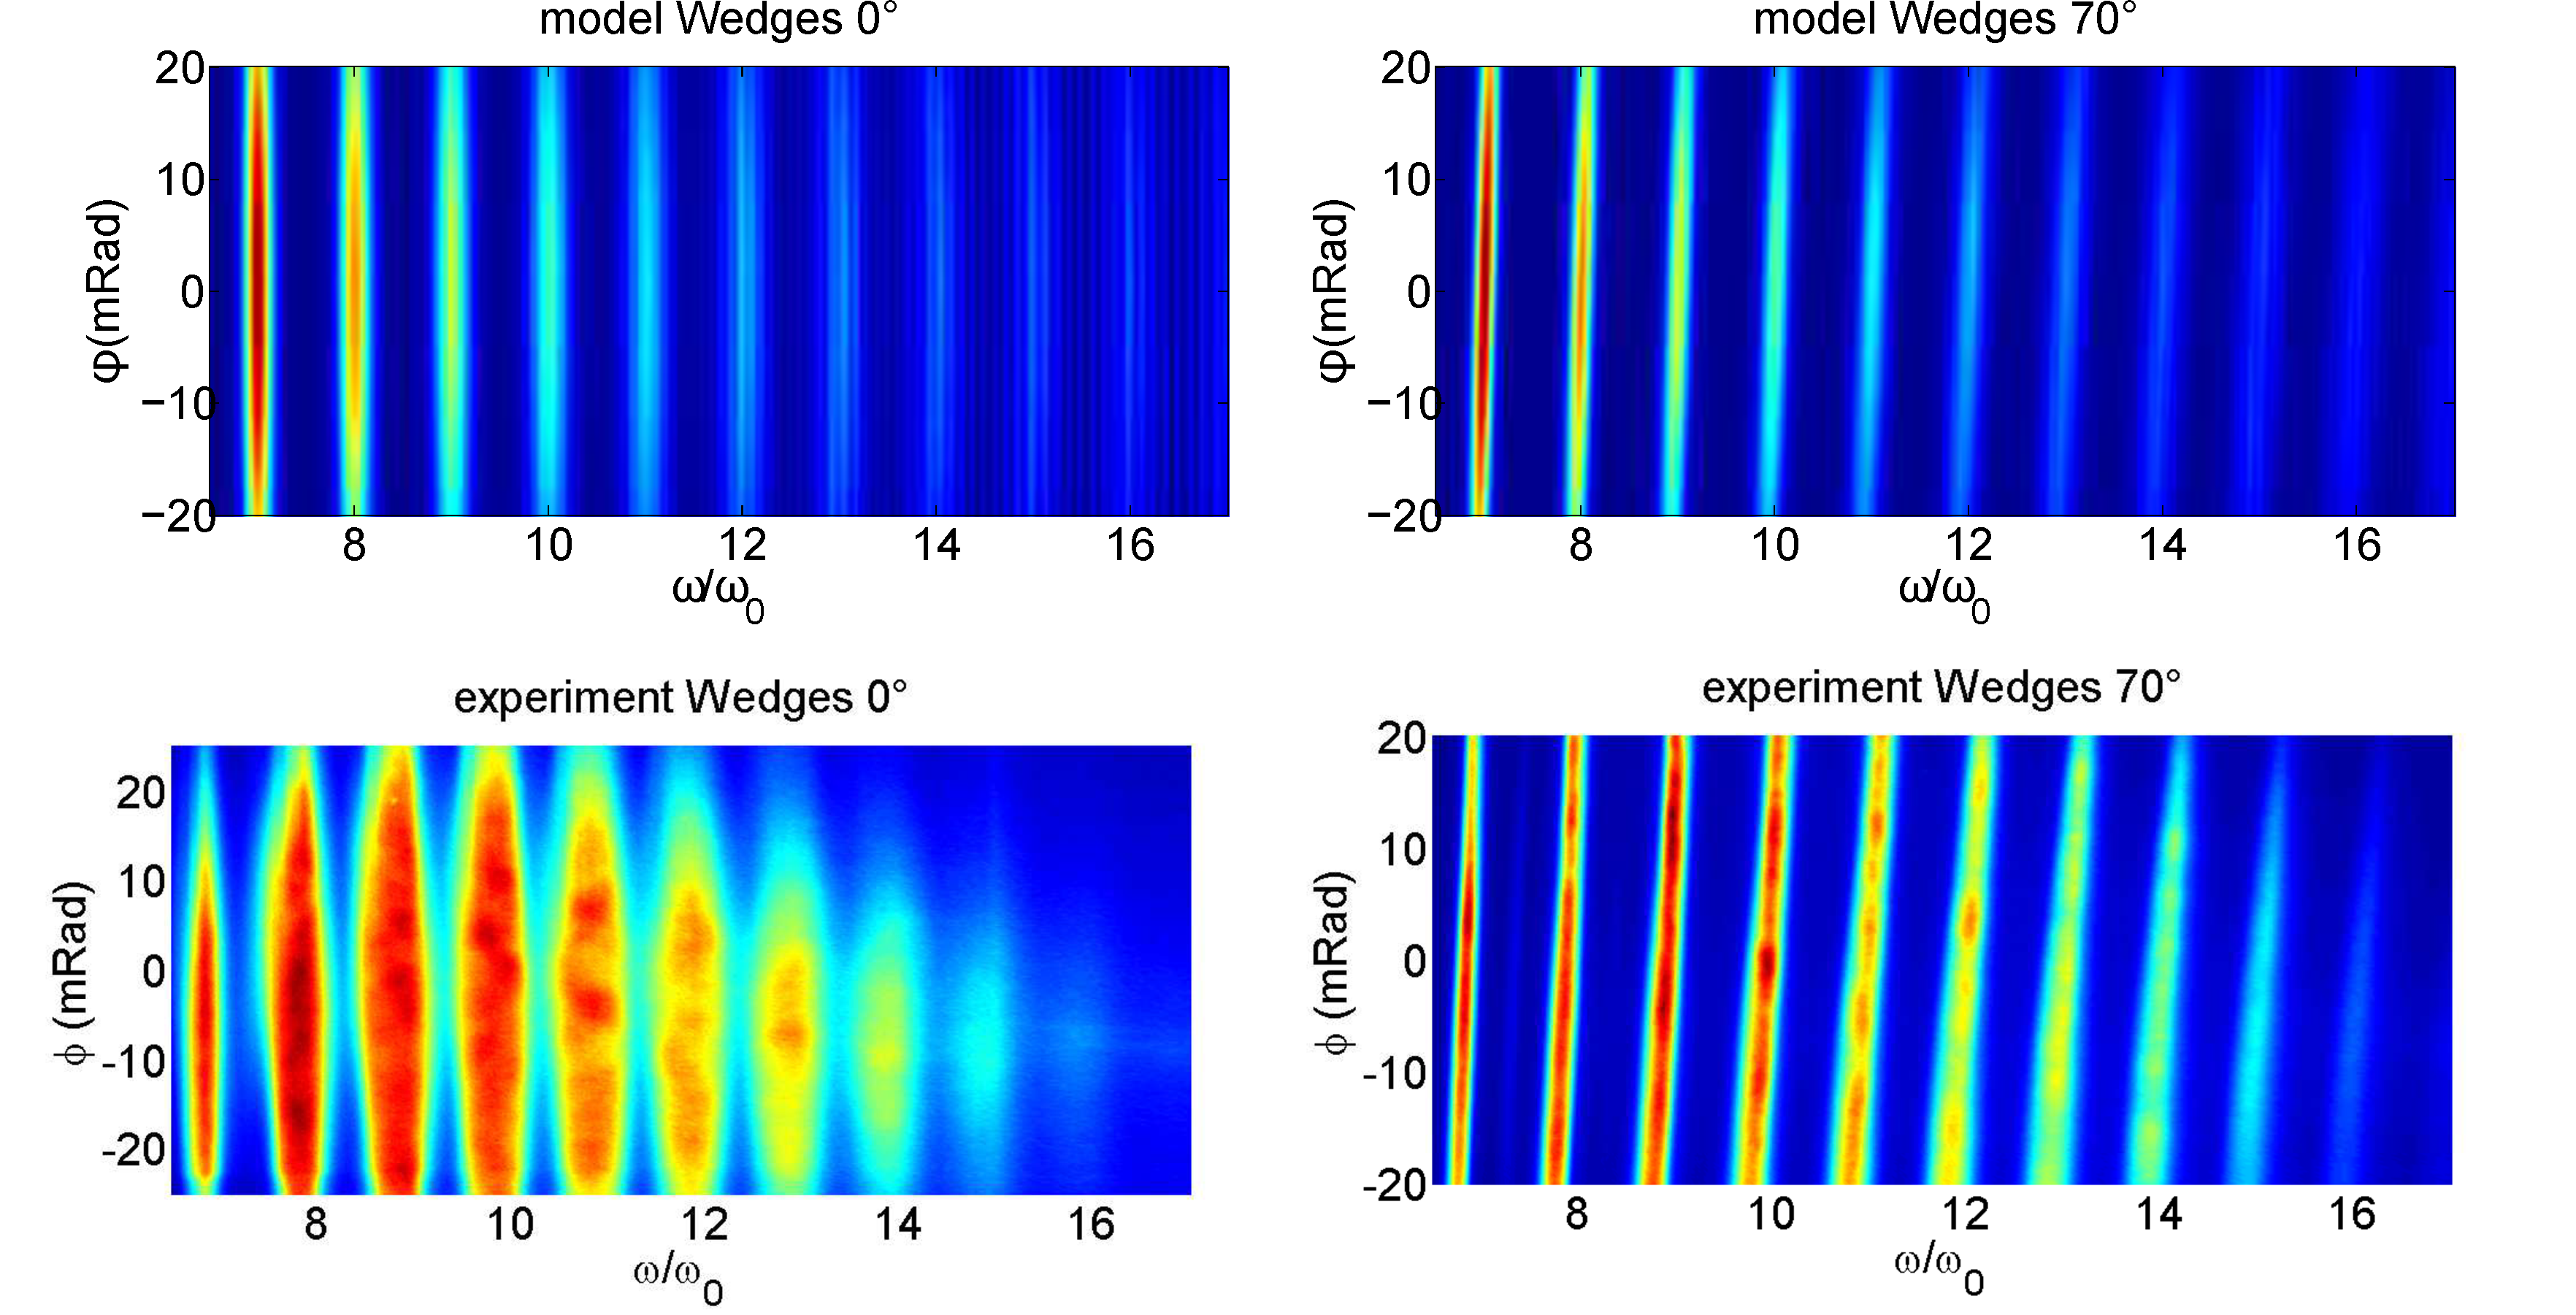
\includegraphics[width =\textwidth]{../chapitre6/images/synthese_scanWFR_a0=0p1_exp_a0=0p4_simu.pdf}\\
\caption{\label{fig:hhgfield_verticalspectral} Simulated (top) and experimental (bottom) influence of WFR on harmonic spectra for $a_0 = 0.1$ .}%and the simulation for $a_0 = 0.5$ 
\end{figure}


\noindent \g{Influence of gradient expansion:}\\
\noindent As the plasma expands, the intrinsic harmonic femtosecond chirp is expected to increase. Consequently in the experiment, the harmonics are expected to" bend"  with pump-probe delay. This is what we observe as can be seen in the screen shot of angular X-UV emission spectra measured for pump-probe delays between -0.1ps and 0.7ps represented in Fig~\ref{fig:AttoFrog_influenceDelay_20140811l}, for a  prepulse intensity is $\sim 10^{14}\,\mathrm{W/cm^2}$. Note that this observation is not so straightforward after $0.5\,\mathrm{ps}$. Indeed, this experiment was very challenging because of the pump/probe spatial overlap fluctuations. For this reason, this result is only preliminary and no quantitative information have been computer from it. We plan to actively stabilize the pump/probe overlap in our future experiment.\\

\noindent To conclude, we have demonstrated that controlled WFR of the driving laser pulse at focus allows one to perform a time-to-space mapping of the attosecond train by means of wavefront rotation of the driving laser pulse. 
This idea was implemented in the ``attosecond lighthouse''~\cite{Wheeler2012} with the difference that here, the attosecond pulses are not fully separated in the vertical direction. This principle is called "gating" and has already been investigated both theoretically and experimentally~\cite{TheseHenri,TheseSylvain}.
Temporal gating is used in FROG measurement techniques~\cite{Trebino1993} in order to fully characterize the temporal profile of optical laser pulses. By varying the relative delay between the gate and the pulse under study and measuring its spectrum, one builds a spectrogram that allows us to fully reconstruct the temporal pulse profile. We will discuss hereafter the possibility of applying such a technique to attosecond streaking in order to perform an ``attosecond FROG''.

\begin{figure}[H]
\centering
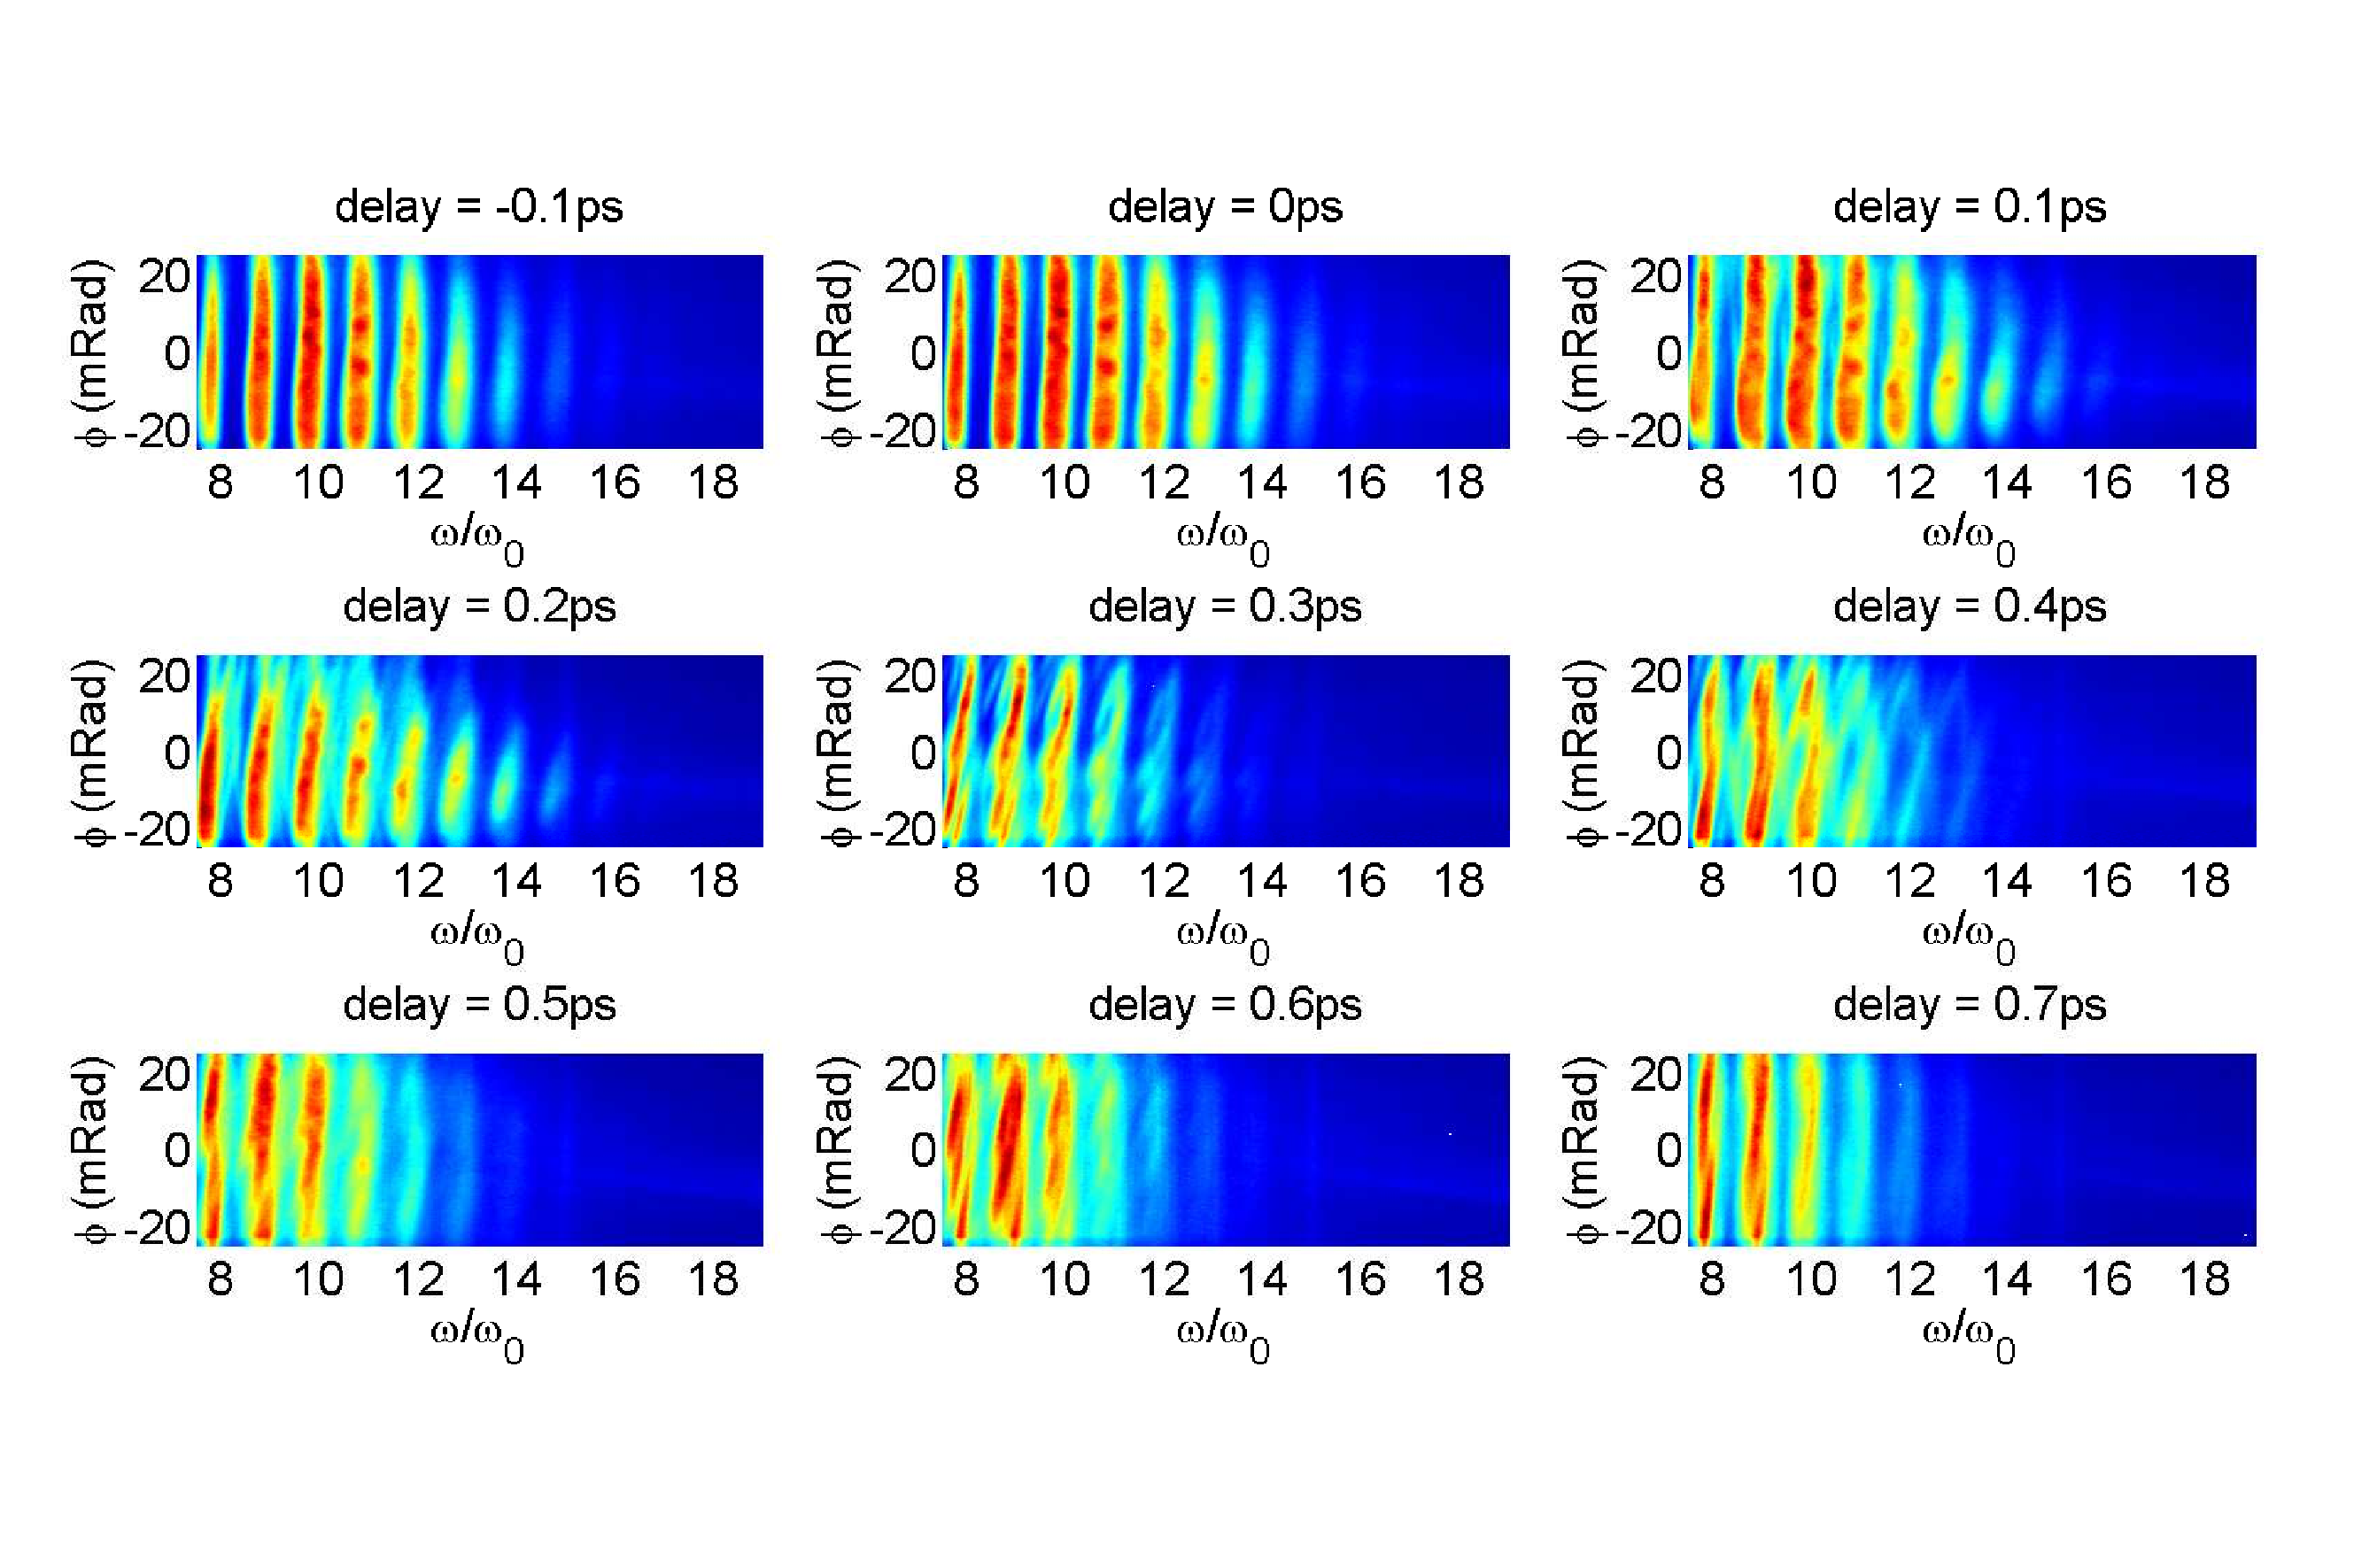
\includegraphics[width =\textwidth]{../chapitre6/images/AttoFrog_influenceDelay_20140811.pdf}\\
\caption{\label{fig:AttoFrog_influenceDelay_20140811l} Angularly-resolved harmonic spectra recorded on the MCP with WFR. The prepulse intensity is $\sim 10^{14}\,\mathrm{W/cm^2}$.}%and the simulation for $a_0 = 0.5$ 
\end{figure}

%the second wedge is turned by $50^{\circ}$











%\begin{figure}[H]
%\makebox[\textwidth][c]{
%\includegraphics[width =0.9\textwidth]{../chapitre6/images/effectOgWFR_atfocus.pdf}}
%\caption{\label{fig:effectOgWFR_atfocus} $a_0 = 0.1$}
%\end{figure}
%
%
%\begin{figure}[H]
%\makebox[\textwidth][c]{
%\includegraphics[width =0.9\textwidth]{../chapitre6/images/effectOgWFR_atfocus_1mJ.pdf}}
%\caption{\label{fig:effectOgWFR_atfocus_1mJ} $a_0 = 0.15$ }
%\end{figure}





\section{Basic principle of attosecond FROG retrieval}

Following Trebino's notation \cite{Trebino1993}, a FROG trace is defined by the following expression:

\begin{equation}
\label{eq:equationFrog0}
I_{FROG}(\omega,\tau) = |\int_{t\in \mathbb{R}}E(t)g(t-\tau)e^{-i\omega t}dt|^2
\end{equation}

\noindent where $E$ is the electric field to be measured, $g$ the gate function. Inverting the FROG trace, that is to say reconstructing $E$ knowing $I_{FROG}$, is a type of inversion problem that has been extensively studied in various fields of science such as holography, astrophysics and biology. We describe in more details the required conditions for this inversion to be possible in Section~\ref{ch:Measuring the gradient expansion}. Inversion of Eq~\ref{eq:equationFrog0} is possible using a FROG retrieval algorithm converging to a (very often) unique solution. Let us adapt the algorithm to the attosecond streaking case. \\

\noindent \g{Spectrogram in the case of attosecond streaking:}

\noindent Unlike Trebino's definition of a FROG trace, the field $E_{hhg}(\theta_y,t)$ to reconstruct is two- dimensional. When turning a wedge, angular dispersion $\beta$ is no longer $0$ such that we can assess the following relation for the harmonic field:

$$
E_{hhg,\beta}(\theta_y,t)= E_{hhg,\beta=0}(\theta_y-v_{rot} t,t)
$$

\noindent where $E_{hhg,\beta=0}$ denotes the harmonic field in absence of WFR, and $E_{hhg,\beta}$ after we introduce WFR with velocity $v_{rot}$. Using this empirical relation, this leads to the definition of the following spectrogram:

\begin{equation}
\label{eq:equationFrogAtto}
I_{FROG}(\omega,\theta_y) = |\int_{t\in \mathbb{R}}E_{hhg,\beta=0}(\theta_y-v_{rot} t,t)e^{-i\omega t}dt|^2
\end{equation}

\noindent One clearly sees the problem we are faced with so far: in order to write $I_{FROG}$ in the form of a FROG trace, as defined by Trebino, and therefore reconstruct the field using a singular value decomposition (SVD) inversion algorithm~\cite{Kane2008}, one needs to write $E_{hhg,\beta=0}$ as the product of a temporal function with a spatial envelop, that is to say neglect all spatio-temporal couplings:
\begin{equation}
\label{eq:SperationCondition}
E_{hhg,\beta=0}(\theta_y,t)= g(\theta_y) E_{hhg,\beta=0}(0,t)
\end{equation}

\noindent Which means the spectrogram writes:

\begin{equation}
\label{eq:equationFrogAtto2}
I_{FROG}(\omega,\theta_y) = |\int_{t\in \mathbb{R}}E_{hhg,\beta=0}(0,t)g(\theta_y-v_{rot} t)e^{-i\omega t}dt|^2
\end{equation}



\noindent In Fig~\ref{fig:generatedField}, we implemented the SVD algorithm on a numerically generated attosecond pulse train, where the condition \ref{eq:SperationCondition} was met, and show the successful reconstruction with a error $<0.5$\% in Fig~\ref{fig:generatedField}.


\begin{figure}[H]
\makebox[\textwidth][c]{
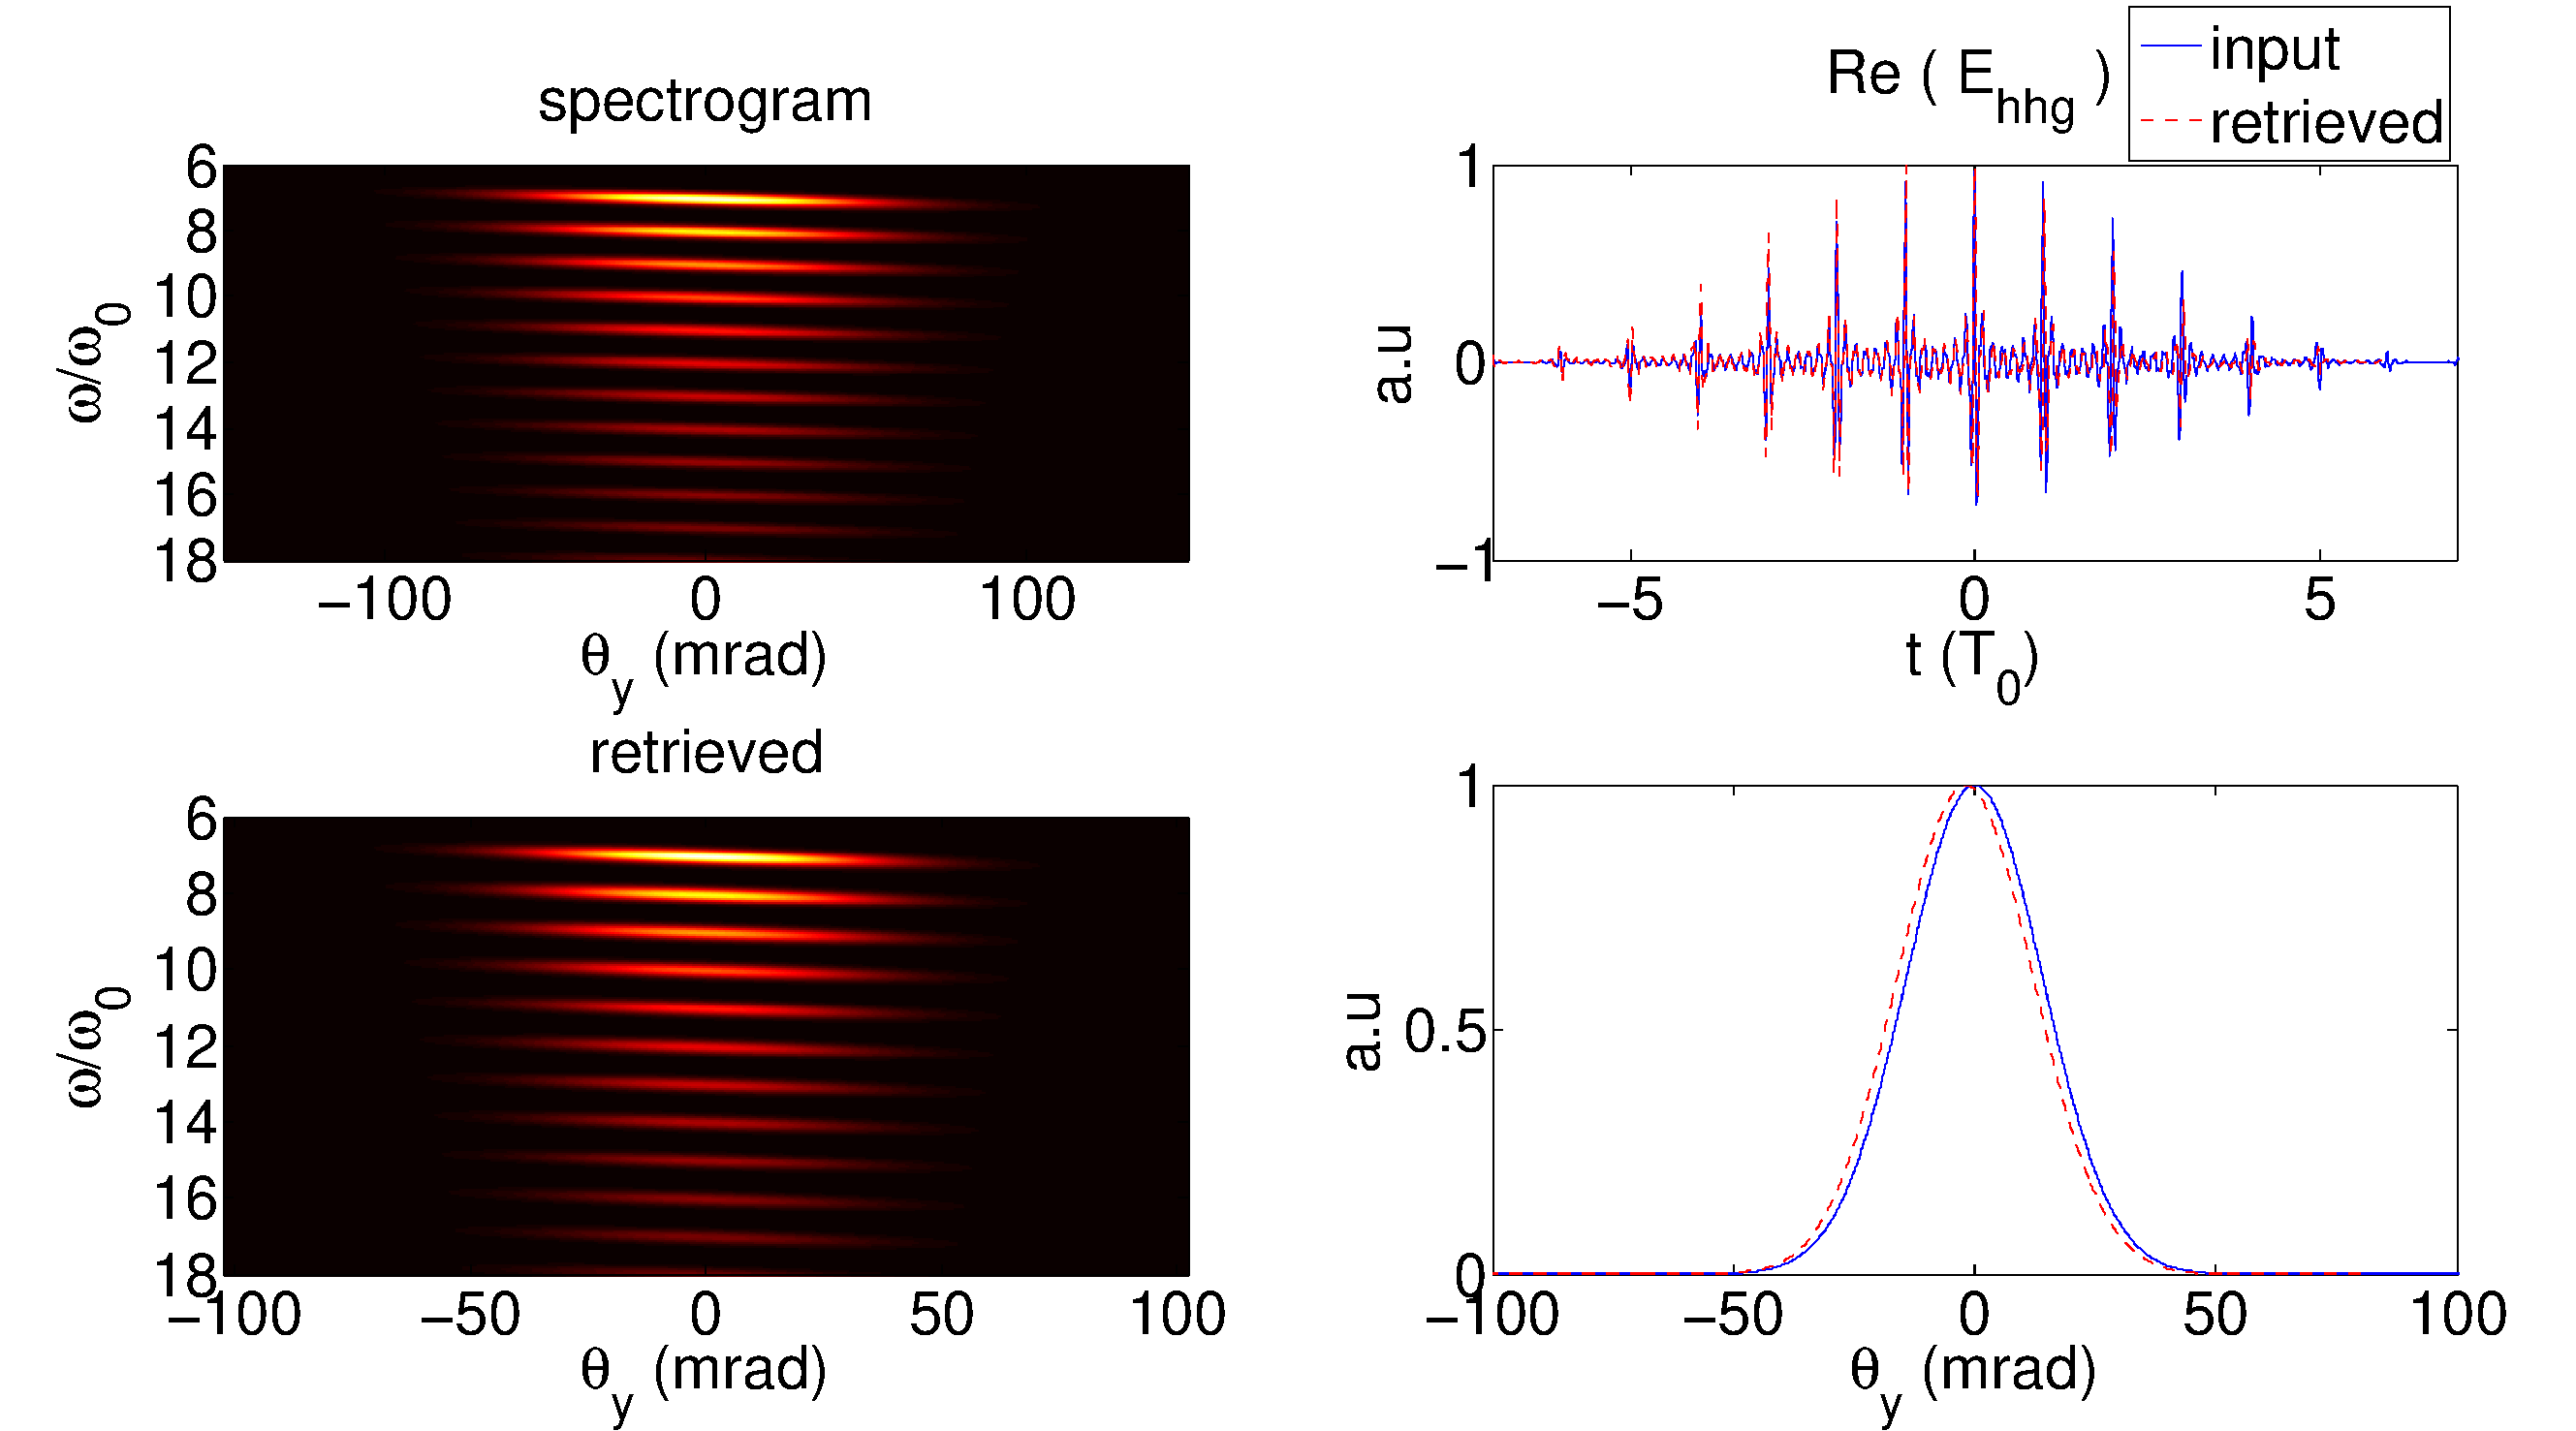
\includegraphics[width =1.1\textwidth, height = 10cm]{../chapitre6/images/generatedField.pdf}}
\caption{\label{fig:generatedField} Result of iterative SVD FROG algorithm for input trace generated using $V_{rot} = -2 \,\mathrm{mrad/[T_0]}$, where the residual error is $<0.5\%$. The initial harmonic field is represented in blue (top right), where we superimposed in red the retrieved field after 500 iterations. The corresponding gate is represented in the bottom right plot.}
\end{figure}

\noindent Unfortunately, running the reconstruction on the experimental data was not possible for the reasons described in the following paragraph. \\

\noindent \g{Experimental limitations of the method:}

We ran the SVD algorithm on our experimental traces shown on Fig~\ref{fig:effectOgWFR_atfocus_1mJ}, and found retrieved errors of the order of several percent, which were too high to consider this measurement as an actual characterization of the attosecond pulse train. Several reasons can account for the bad reconstruction:


\begin{itemize}
\item The signal recorded on the MCP did not show the whole distribution of the harmonic spectrum. The signal was cut at the edges because of the limited angular range of detection. This can be addressed by relaxing the focusing condition to get a larger waist, and therefore decrease the divergence of the harmonics. It will be implemented  in future experiments.
\item The reconstruction is intrinsically dependent on the exact measurement of $v_{rot}$ which would require us to characterize the phase of the IR pulse in addition to the spectrum in the focusing plane. We plan to perform full spatio-temporal characterization of our focused laser using the "Thermite"~\cite{miranda2014spatiotemporal,pariente2015measuring} technique to address this problem.
\item The signal/noise ratio --visible on some images in Fig~\ref{fig:effectOgWFR_atfocus_1mJ}--  is always a limitation when the reconstruction is based on phase retrieval. This problem is partially solved by adding filters to our imaging system and pulsing the MCP detection, but all ambient radiation sources degrading the harmonic signal remain under investigation.
\begin{figure}[H]
\makebox[\textwidth][c]{
\includegraphics[width =0.9\textwidth]{../chapitre6/images/effectOgWFR_atfocus_1mJ.pdf}}
\caption{\label{fig:effectOgWFR_atfocus_1mJ} Experimental attosecond FROG traces for $a_0 = 0.15$. Top: Laser spectrum is apodized which yields to a compressed pulse of $30\,\mathrm{fs}$, Bottom: compressed laser to $23\,\mathrm{fs}$ (see Chapter~\ref{chapter:Overall presentation of the laser system} for description of apodisation method)}
\end{figure}
\end{itemize}




\noindent One should now consider a more fundamental limitation to this measurement technique, which is intrinsically related to the implementation of the algorithm.
Indeed, we made the hypothesis that the harmonic field could be written as the product of a spatial profile with a temporal profile. In practice, there is no rigorous justification allowing for this separation-of-variables. In particular, spatio-temporal coupling of the laser beam due to inhomogeneous compression, inhomogeneous spatial distribution of a prepulse (and therefore inhomogeneous gradient expansion) will directly affect the phase front of the harmonic profile. 

\noindent In a final observation on these limitations, it would be necessary to implement a retrieval where (i) $v_{rot}$ does not need to be accurately calibrated and (ii) the full two-dimensional profile $E_{hhg,\beta=0}(\theta_y,t)$ is reconstructed, as opposed to its value in $\theta_y =0$. This goes beyond the scope of the work presented here but constitutes an interesting theoretical challenge.




\section{Conclusion}

We have performed a series of experiments validating the harmonic emission properties from plasma mirrors already demonstrated in the literature~\cite{thaury2010high,thaury2008coherent,TheseSylvain,TheseArnaud,theseAnto,TheseHenri}, namely how each attosecond pulse emission time depends on the temporal structure of the driving laser pulse~\cite{thaury2010high,theseAnto,TheseArnaud}. The HHG emission is coherent and phase-locked to the driving laser intensity and phase profile. We have shown how the spectral components of the X-UV light depends on the spatial intensity distribution of the driving laser. This then led us to study the feasibility of an "attosecond FROG" type measurement by controlling the angular chirp of the main laser pulse, and observing the subsequent tilt of the harmonic lines in the angularly resolved emission spectra. This effect can be fully predicted by a simple one-dimensional model used to calculate the emission time at each position of the laser across the laser focus with WFR. We have implemented an SVD retrieval algorithm similar to that used for standard FROG retrieval of IR laser pulses. However, our approach is limited: the quality of the images has to be improved, the driving laser has to be fully characterized at focus, and most of all, the retrieval algorithm should be made independent of the laser WFR. 































